\chapter{Proceso de desarrollo}
\label{ch:desarrollo}
Este capítulo abarca mi parte de desarrollo de software de la aplicación web de SmartU. Se describe el análisis y los requisitos que hemos obtenido para este sistema, pasando por el diseño e implementación del mismo. Al final del capítulo se incluye un apartado de herramientas que han sido utilizadas para el desarrollo de este software.

\section{Introducción}
Al comenzar el desarrollo, se pudo apreciar que había una alta posibilidad de sufrir cambios a lo largo del proceso debido a que el alcance del mismo no estaba muy delimitado. Es por ello que se optó por seguir una metodología principalmente ágil, la cual permitía mayor flexibilidad y facilidad para adaptar posibles cambios.\\

En el desarrollo ágil es importante la comunicación entre todos los miembros del equipo y que éstos, de alguna forma, participen activamente durante el desarrollo. No todos los miembros de este equipo multidisciplinar trabajan en el ámbito de la Ingeniería Informática, pero sabíamos que podían colaborar en las primeras fases aportando ideas y posibles requisitos. Sin embargo, sí que era importante que hubiera comunicación y consenso entre los miembros del área de Informática. Con mi compañero Emilio se realizó una puesta en común para intentar unificar las plataformas que cada uno teníamos que desarrollar.\\

Siguiendo algunos de los principios del desarrollo ágil, se ha evitado realizar documentación innecesaria, y se ha optado por ir a lo primordial y esencial, sin que ello repercuta en la calidad del software. Hay que tener en cuenta que este desarrollo pretende ser continuado y mejorado en el tiempo, por lo que una documentación base correcta es importante.\\

Por último, añadiremos que se ha preferido optar por establecer una lista de requisitos del sistema en lugar de emplear la técnica de las \textbf{historias de usuario}, ya que no son de obligado cumplimiento el desarrollarlas, y se ha de tener en cuenta el hecho de que el desarrollo será continuado por otras personas en el futuro.

\section{Análisis}
La fase de análisis se distribuye en \textbf{dos grandes bloques}:

\begin{itemize}
    \item El primer bloque comprende el análisis en equipo del problema y la extracción de unos primeros requisitos y usuarios base sobre los que basaremos nuestras decisiones futuras a la hora de desarrollar el sistema. Aquí se realizarán diversas técnicas de generación de ideas y prototipado para acotar y definir mejor el sistema.
    \item El segundo bloque es más habitual del proceso de desarrollo de software, ya que se va a dedicar a recopilar y mostrar los requisitos del sistema ya definidos correctamente, tras haber terminado el análisis del primer bloque.
\end{itemize}

\subsection{Generación de ideas y extracción de requisitos}
Tal y como se describió en el capítulo \ref{ch:metodologia}, es importante realizar sesiones de generación de ideas para empezar a recopilar ideas para el desarrollo. Se realizó un seminario sobre tecnologías emergentes, y otro sobre \textit{Design Thinking/Brainstorming}. Esto se describe con más detalle en el capítulo \ref{ch:conclusiones}.\\

Más adelante se obtuvo más información gracias a la presentación del proyecto multidisciplinar que se hizo en la Facultad de Ciencias de la Actividad Física y del Deporte, realizada por los compañeros Javier y Juan. Allí se pudo enseñar el proyecto a potenciales usuarios (\textit{stakeholders}) y recibimos opiniones muy interesantes de posibles características que les gustaría ver para que fuese una aplicación web más completa y funcional.

\subsubsection{Usuarios del sistema}
Tras las reuniones de generación de ideas, se llegó a la siguiente conclusión respecto a \textbf{quiénes son los usuarios potenciales del sistema}. Es importante poder definir a los posibles futuros usuarios de nuestra aplicación para así poder enfocar mejor los requisitos y el diseño de nuestra aplicación web. Nuestro equipo en si consta de algunos de ellos: son los estudiantes y profesores, o en general, la comunidad educativa.

\begin{itemize}
    \item Los \textbf{estudiantes} son potenciales usuarios registrados de nuestra aplicación web. Podemos concretar más e irnos al segmento de estudiantes de último año de grado o máster que necesitan una idea para realizar un proyecto de final de grado/máster, pero también están aquellos estudiantes que cuentan con una idea para un proyecto y necesitan a otros estudiantes con los que conformar un equipo.\\
    Este grupo de usuarios es el que se prevee que sería el que utilizase el sistema con mayor frecuencia.
    \item Otro segmento de usuarios es los \textbf{habitantes de la ciudad}. La diferencia radica en que por lo general, es un colectivo no asociado a la universidad y desconocedor de lo que ocurre dentro de ésta. Por ello, no son considerados potenciales usuarios que se van a registrar en el sistema, pero si entrarán y consultarán las ideas que se han publicado.\\
    Pueden ser participantes activos de un proyecto que se esté creando si éste es un proyecto que le interese o afecte a su entorno (barrio, movilidad, economía, etc).
    \item Por último, tenemos el grupo de \textbf{usuarios empresarios}. Estos son aquellas personas que, o bien tienen una idea, o encuentran interesante una idea que han visto publicada en la aplicación. Pueden ponerse en contacto con un equipo de un proyecto y ayudarles con financiación o promoción de su idea, entre otras posibilidades.
\end{itemize}

Para representar de una forma más visual a estos usuarios, se han creado una serie de bocetos de usuario (o \textit{User Persona}), que esquematizan y ayudan a definir de un vistazo el tipo de perfil de usuario que hemos definido. Podemos verlos en las figuras \ref{usuario_estudiante}, \ref{usuario_ciudadano} y \ref{usuario_empresario}.\\

Como podemos ver, el conjunto de potenciales usuarios intenta abarcar a todo el conjunto de la población, por lo que una buena implantación del mismo podría \textbf{reportar enormes beneficios} para todos ellos, ya sea encontrando un proyecto en el que trabajar, como llevar a cabo una idea que mejore la vida en general de los ciudadanos.

\begin{figure}
    \centering
    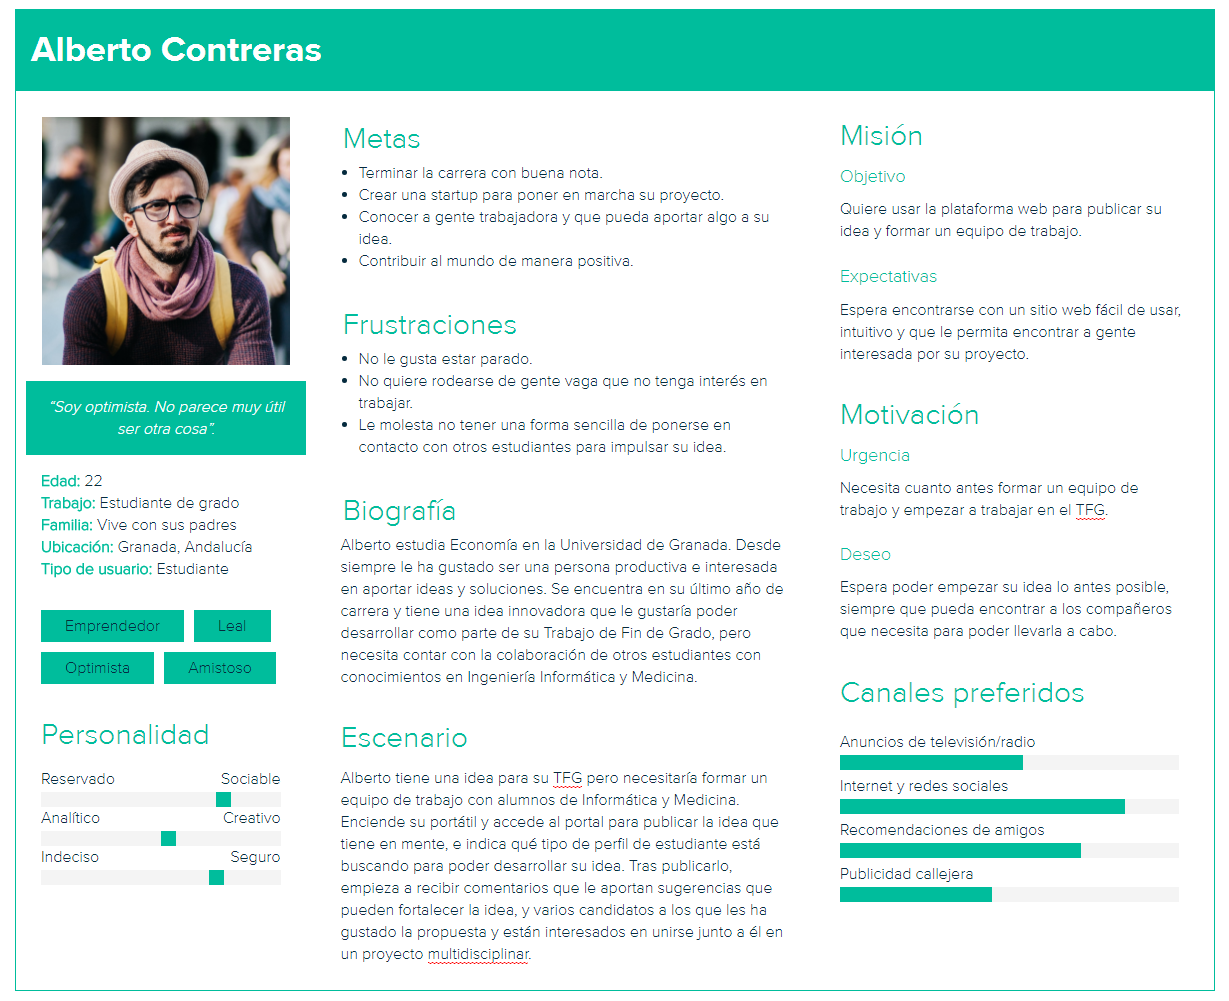
\includegraphics[scale=0.275]{usuario_estudiante}
    \caption{\textit{User Persona} de un estudiante}
    \label{usuario_estudiante}
\end{figure}

\begin{figure}
    \centering
    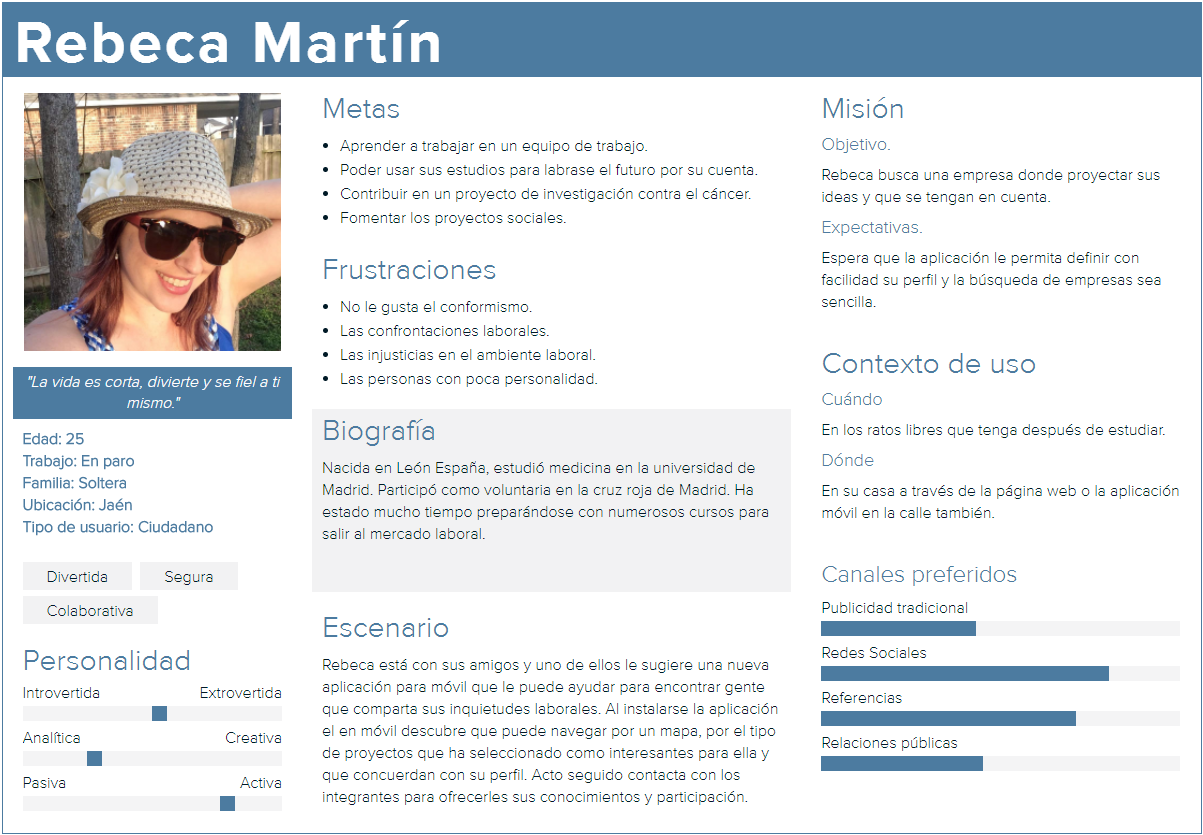
\includegraphics[scale=0.275]{usuario_ciudadano}
    \caption{\textit{User Persona} de un ciudadano}
    \label{usuario_ciudadano}
\end{figure}

\begin{figure}
    \centering
    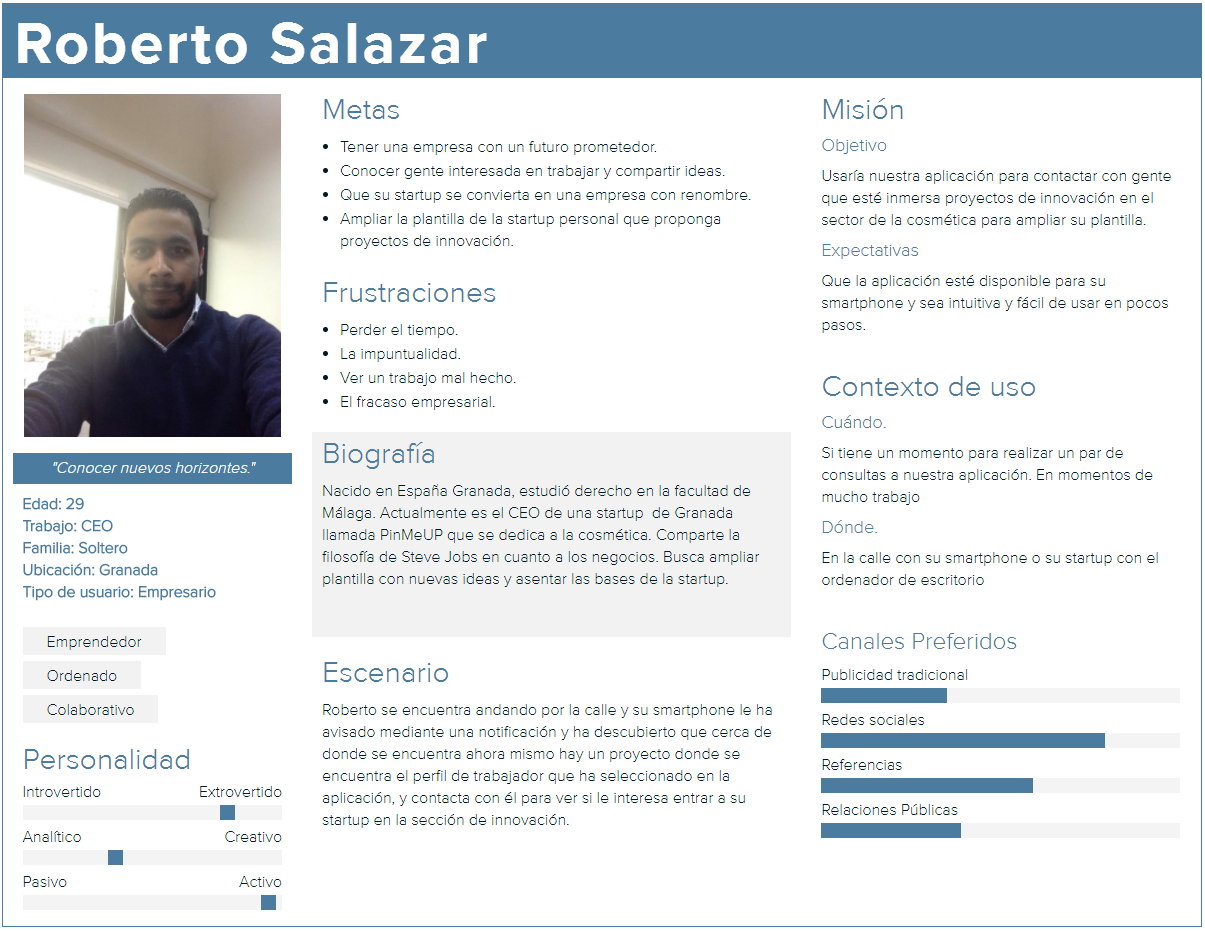
\includegraphics[scale=0.275]{usuario_empresario}
    \caption{\textit{User Persona} de un empresario}
    \label{usuario_empresario}
\end{figure}

\subsection{Requisitos del sistema}
En base a todas las reuniones e información recabada de las mismas y de posibles stakeholders, se ha confeccionado la siguiente lista de requisitos del sistema.

\subsection*{Requisitos de datos}
Se quiere implementar un sistema de información basado en web que sea capaz de almacenar la información relativa a proyectos para la universidad, permitiendo la asignación de información más detallada como área de conocimiento del proyecto, descripción y avances del mismo, así como la información perteneciente a los usuarios que se registren en la plataforma, sus comentarios e información de perfil.

\begin{description}
    \item[RD1. Proyecto:] Un proyecto necesita almacenar la siguiente información:
        \begin{description}
            \item[Nombre:] Cadena de caracteres.
            \item[Descripción:] Cadena de caracteres.
            \item[Página web:] Cadena de caracteres.
            \item[Localización:] Cadena de caracteres.
            \item[Coordenadas:] Cadena de caracteres.
            \item[Fecha de creación:] Fecha de alta del proyecto en el sistema.
            \item[Fecha de eliminación:] Fecha estimada de finalización del proyecto.
            \item[Fecha de actualización:] Fecha de última actualización del proyecto.
            \item[Propietario:] Identificador del usuario registrado que creó el proyecto.
            \item[Imagen destacada:] Cadena de caracteres del nombre de un archivo de imagen.
        \end{description}
    \item[RD2. Redes sociales:] Los proyectos y los usuarios pueden definir sus propias redes sociales para darse a conocer, y necesitan la siguiente información:
        \begin{description}
            \item[Nombre:] Cadena de caracteres.
            \item[URL:] Cadena de caracteres.
            \item[ID de usuario:] Identificador del usuario.
            \item[ID del proyecto:] Identificador del proyecto.
        \end{description}
        Una red social petenece a un usuario o a un proyecto, se han unificado para evitar redundancia.
    \item[RD3. Área del proyecto:] Los proyectos tienen una o varias áreas, y se necesita la siguiente información para poder guardarlas.
        \begin{description}
            \item[Nombre:] Cadena de caracteres.
            \item[Descripción:] Cadena de caracteres.
        \end{description}
    \item[RD4. Buena Idea:] Una buena idea se asemeja a un ``Me gusta'' de redes como Facebook o Twitter. Necesita la siguiente información:
        \begin{description}
            \item[ID del proyecto:] Identificador del proyecto.
            \item[ID del usuario:] Identificador del usuario.
            \item[Tipo:] Indica el tipo de recurso al que se le da ¡Buena Idea!, pensado para ampliar esta funcionalidad a otro tipo de recursos.
            \item[Borrado:] Indica si el ¡Buena Idea! dado se quitó o no.
        \end{description}
    \item[RD5. Especialidad:] La especialidad es algo a lo que un usuario se dedica o que tiene experiencia en ello. Sirve para encontrar a gente de un determinado campo que necesita un proyecto. Se necesita la siguiente información:
        \begin{description}
            \item[Nombre:] Cadena de caracteres.
            \item[Descripción:] Cadena de caracteres.
        \end{description}
    \item[RD6. Experiencia en especialidad:] Partiendo del requisito de dato anterior, un usuario cuenta con un cierto nivel de experiencia en una especialidad, lo cual requiere almacenar la siguiente información:
        \begin{description}
            \item[Experiencia:] Cadena de caracteres.
            \item[ID de la especialidad:] Identificador de la especialidad.
            \item[ID del usuario:] Identificador del usuario.
        \end{description}
    \item[RD7. Comentario:] Los usuarios registrados pueden dejar comentarios en sus proyectos o en los de otros usuarios. Se necesita la siguiente información:
        \begin{description}
            \item[Contenido:] Cadena de caracteres.
            \item[Fecha de creación:] Fecha insertada cuando se creó el comentario.
            \item[ID del usuario:] Identificador del usuario que hace el comentario.
            \item[ID del proyecto:] Identificador del proyecto donde se comenta.
        \end{description}
    \item[RD8. Avance:] Un proyecto puede tener un conjunto de avances que muestre a los usuarios el progreso que se está logrando con el proyecto. Necesita la siguiente información:
        \begin{description}
            \item[Nombre:] Cadena de caracteres.
            \item[Descripción:] Cadena de caracteres.
            \item[Fecha de creación:] Fecha de publicación del avance
            \item[Imagen destacada:] Cadena de caracteres del nombre de un archivo de imagen.
            \item[ID del proyecto:] Identificador del proyecto al que va asociado.
        \end{description}
    \item[RD9. Vacante:] Una vacante representa una disponibilidad de un puesto, en una determinada disciplina, como integrante en un proyecto. Se necesita la siguiente información:
        \begin{description}
            \item[Experiencia:] Una cadena de caracteres.
            \item[Especialidad:] Un identificador de una especialidad concreta.
        \end{description}
    \item[RD10. Hashtag:] Uno o varios proyectos pueden tener etiquetas conocidas como \textit{hastags}, y se necesita guardar para ello:
        \begin{description}
            \item[Nombre:] Una cadena de caracteres.
        \end{description}
    \item[RD11. Usuario:] Un usuario necesita almacenar la siguiente información:
        \begin{description}
            \item[Nombre:] Cadena de caracteres.
            \item[Apellidos:] Cadena de caracteres.
            \item[Email:] Cadena de caracteres.
            \item[Contraseña:] Cadena de caracteres.
            \item[Biografía:] Cadena de caracteres.
            \item[Página web:] Cadena de caracteres.
            \item[Localización:] Cadena de caracteres.
            \item[Puntos:] Número entero.
            \item[CIF:] Cadena de caracteres.
            \item[Admin:] Booleano.
            \item[Verificado:] Booleano.
            \item[Avatar:] Cadena de caracteres del nombre de un archivo de imagen.
        \end{description}
    \item[RD12. Solicitud colaboración:] Los usuarios pueden solicitar colaborar en un proyecto que tenga vacantes disponibles. Se necesita almacenar la siguiente información:
        \begin{description}
            \item[Fecha:] Fecha de creación de la solicitud.
            \item[Descripción:] Una cadena de caracteres.
            \item[Usuario solicitante:] Identificador del usuario que solicita colaborar.
            \item[Proyecto solicitado:] Identificador del proyecto en el que se desea colaborar.
        \end{description}
    \item[RD13. Colaborador:] Un usuario puede ser colaborador de un proyecto en una determinada especialidad. Se necesita almacenar:
        \begin{description}
            \item[ID del usuario:] Identificador del usuario colaborador.
            \item[ID del proyecto:] Identificador del proyecto donde colabora.
            \item[ID de especialidad:] Identificador de la especialidad del colaborador.
        \end{description}
    \item[RD14. Intereses:] Los usuarios pueden marcar intereses en determinadas áreas. Para ello se necesita guardar:
        \begin{description}
            \item[ID del usuario:] Identificador del usuario que marca un interés.
            \item[ID del área:] Identificador del área donde el usuario marca un interés.
        \end{description}
    \item[RD15. Status:] Un ususario puede tener un status en base a su participación en la aplicación web, por ejemplo publicando proyectos o bien dando ``Buena Idea'' a otros. Se requiere la siguiente información:
        \begin{description}
            \item[Nombre:] Cadena de caracteres. Es el nombre que recibe el status.
            \item[Puntos:] Número entero que representa los puntos que se han de alcanzar para llegar a dicho status.
        \end{description}
    \item[RD16. Seguidor:] Un usuario puede seguir a otro para estar al tanto de sus proyectos y de lo que hace en la aplicación web. Se necesita almacenar lo siguiente:
        \begin{description}
            \item[ID del usuario seguido:] Identificador del usuario al que se sigue.
            \item[ID del usuario seguidor:] Identificador del usuario que está siguiendo.
        \end{description}
\end{description}

\subsection*{Restricciones semánticas}
\begin{description}
    \item[RS1.] Un usuario no registrado no puede participar en la aplicación web salvo para consultar la información.
    \item[RS2.] Un usuario no puede tener el mismo email o nombre de usuario que otro registrado anteriormente.
    \item[RS3.] Un proyecto solo puede tener un usuario propietario.
    \item[RS4.] Los usuarios solo pueden modificar o eliminar proyectos de los que son propietarios.
    \item[RS5.] Un usuario puede solicitar unirse al proyecto si hay vacantes y si no es ya propietario o colaborador.
    \item[RS6.] Un usuario no puede seguirse a sí mismo.
    \item[RS7.] Un usuario no puede dar Buena Idea a su/s propio/s proyecto/s.
    \item[RS8.] Los usuarios con correo corporativo reconocido serán registrados automáticamente como usuarios ``verificados''.
\end{description}

\subsection*{Requisitos funcionales}
\subsubsection{Requisitos funcionales de inserción}
\begin{description}
    \item[RF1. Registrar usuario:] un usuario invitado puede registrarse en el sistema para poder utilizar el resto de funcionalidades.
    \item[RF2. Crear proyecto:] Un usuario registrado puede crear un nuevo proyecto en el sistema para dar a conocer su idea.
    \item[RF3. Dar Buena Idea:] Un usuario puede dar un Buena Idea a un proyecto
    \item[RF4. Dejar un comentario:] Un usuario registrado puede dejar un comentario en un proyecto.
    \item[RF5. Elegir áreas de interés:] Un usuario registrado puede seleccionar una o más áreas que sean de su interés para encontrar proyectos afines.
    \item[RF6. Seguir a un usuario:] Un usuario registrado en el sistema puede seguir a otro usuario para estar al tanto de su actividad en la aplicación.
    \item[RF7. Crear vacante:] Un usuario propietario de un proyecto puede crear una vacante para buscar colaboradores para su proyecto.
    \item[RF8. Solicitar colaboración:] Un usuario puede solicitar colaborar en un proyecto que no sea suyo si éste tiene una vacante disponible.
    \item[RF9. Insertar avance:] Un usuario propietario de un proyecto puede crear un avance de un proyecto que muestre algun tipo de progreso.
    \item[RF10. Insertar nuevo colaborador:] Un usuario propietario de un proyecto puede aceptar o rechazar una petición de colaboración para una vacante.
\end{description}

\subsubsection{Requisitos funcionales de consulta}
\begin{description}
    \item[RF11. Listar solicitudes:] Un usuario propietario de un proyecto puede listar las solicitudes de colaboración en su proyecto pendientes de aprobación.
    \item[RF12. Listar vacantes:] Cualquier usuario puede listar las vacantes existentes para un proyecto.
    \item[RF13. Listar avances:] Cualquier usuario puede listar los avances realizados en un proyecto.
    \item[RF14. Listar proyectos:] Cualquier usuario puede listar los proyectos existentes en la aplicación.
    \item[RF15. Listar usuarios:] Cualquier usuario puede listar usuarios registrados en la aplicación.
    \item[RF16. Listar comentarios:] Cualquier usuario puede listar los comentarios de un proyecto.
    \item[RF17. Listar áreas:] Cualquier usuario puede listar las áreas disponibles en el sistema.
    \item[RF18. Listar colaboradores:] Cualquier usuario puede listar los colaboradores actuales de un proyecto.
    \item[RF19. Consultar detalles de un proyecto:] Cualquier usuario puede ver los detalles de un proyecto.
    \item[RF20. Consultar detalles de un usuario:] Cualquier usuario puede ver el perfil de otro usuario registrado en la aplicación.
\end{description}

\subsubsection{Requisitos funcionales de eliminación}
\begin{description}
    \item[RF21. Eliminar áreas de interés:] Un usuario registrado puede modificar su perfil y eliminar una o varias áreas que sean de su interés.
    \item[RF22. Eliminar Buena Idea de un proyecto:] Un usuario puede eliminar el Buena Idea que le ha dado a un proyecto.
    \item[RF23. Dejar de seguir a un usuario:] Un usuario registrado puede dejar de seguir a otro usuario registrado en el sistema.
\end{description}

\subsection*{Requisitos no funcionales}
\begin{description}
    \item[RNF1.] La aplicación web debe estar finalizada para septiembre de 2017.
    \item[RNF2.] La aplicación web debe tener un diseño adaptable a todo tipo de tamaños de pantalla de dispositivo.
    \item[RNF3.] La aplicación web debe funcionar correctamente en la mayoría de navegadores de Internet más utilizados y en sus últimas versiones disponibles.
    \item[RNF4.] El código de la aplicación debe estar correctamente comentado para facilitar la tarea de mejorarlo a los futuros desarrolladores que continúen el proyecto.
\end{description}

\section{Diseño e Implementación}
Tras el proceso de análisis de nuestro sistema y extracción de los requisitos que necesitaría nuestra aplicación web, procedemos a describir los principales aspectos de diseño e implementación de la misma, incidiendo en aspectos importantes e inherentes al proceso de desarrollo de un sistema de información web.\\

La codificación de la aplicación web de SmartU venía condicionada por la necesidad de un desarrollo que fuese agilizado e iterativo, intentando completar funcionalidades específicas en cada \textit{``paso''} que se diese a lo largo de este proceso. Esto me llevó a tomar una serie de decisiones respecto al lenguage de programación que utilizaría, así como el conjunto de herramientas que me ayudarían con esta tarea, pero siempre teniendo como máxima un desarrollo correcto y bien realizado.

\subsection{Laravel}
Para este proyecto, opté por el framework \textbf{Laravel} \cite{laravel}. La elección del mismo no fue fácil, y llevó algo de tiempo debido al análisis de pros y contras que podría encontrarme a lo largo del proceso de desarrollo. Existen numerosos lenguages de programación como Python, JavaScript, Java, etc, todos con diferentes soluciones de desarrollo web. En el caso de Laravel, se basa en el lenguage PHP, que es ya bien conocido en el mundo de la programación web, y a lo largo de los años ha ido mejorando su potencial con nuevas versiones que incorporaban características que si estaban presentes en otros lenguages.\\

Laravel es un framework de desarrollo web basado en PHP creado por Taylor Otwell en el año 2011. Fue creado con el intento de proporcionar una alternativa más avanzada a \textbf{CodeIgniter}. En muchos lugares de Internet, Laravel es conocido por darle un muy necesitado lavado de cara a PHP, y hacerlo de nuevo más atractivo a la vista de los desarrolladores.\\

Laravel agiliza los procesos en casi todos los apartados existentes del desarrollo de una aplicación web. Proporciona un conjunto de herramientas para gestionar la autenticación de usuarios, bases de datos rutas, entre otros elementos que a continuación se detallan:

\begin{itemize}
    \item Está basado en el conocido patrón de diseño MVC \textbf{(Modelo-Vista-Controlador)}, lo cual permite separar la lógica de nuestra aplicación de la interfaz de usuario, usando como intermediario un controlador que mueva los datos entre modelos y vistas. Con esta idea en mente es fácil obtener un diagrama de clases general del sistema, como el que podemos ver en la imagen \ref{diagramaclases}.
    \item Cuenta con soporte para \textbf{Composer}, lo cual nos permite gestionar de forma sencilla las dependencias de nuestro proyecto, por ejemplo para realizar el despliegue.
    \item Al estar basado en PHP, contamos con el extenso conjunto de funciones que ya nos proporciona el lenguage. Para los programadores actuales de PHP, empezar a usar Laravel \textbf{no supone un mayor esfuerzo}, ya que usa todos los elementos y sintaxis del mismo.
    \item Cuenta con un motor de plantillas, \textbf{Blade}, que permite construir la interfaz web de forma dinámica, recibiendo datos como parámetros y utilizarlos para mostrar la información al usuario.
    \item Laravel dispone de una \textbf{extensa comunidad} de desarrolladores que proporcionan consejos y soluciones a los diversos problemas que puedan surgir a la hora de desarrollar con este framework. En este sentido es fácil encontrar la respuesta a cualquier duda, lo cual hace que el aprendizaje sea mucho más sencillo.
\end{itemize}

\begin{figure}
    \centering
    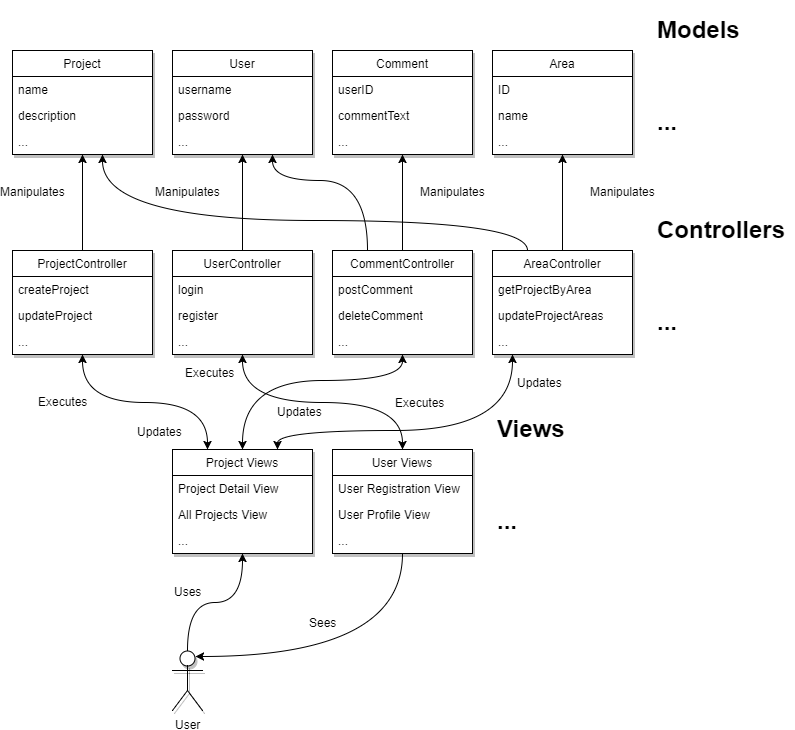
\includegraphics[scale=0.6]{diagramaclases}
    \caption{Diagrama de clases general del sistema}
    \label{diagramaclases}
\end{figure}

La razón por la que elegí este framework era por la sencillez con la que resolvía muchos de los aspectos técnicos que esta aplicación web necesita, además de que se basa en un lenguage de programación que conozco. Siempre es importante estar al tanto de las novedades en los lenguages de programación, pero cuando el tiempo es una restricción muy importante, se hace necesario usar soluciones basadas en algo que ya se conoce. Además, la documentación de este framework es bastante extensa, y cuenta con diversas guías y tutoriales, lo que agillizó bastante su manejo y aprendizaje \cite{laraveldocs}.

\subsection{Estructura del proyecto}
El proyecto se divide en una serie de carpetas generadas automáticamente al crear un nuevo proyecto de Laravel. El código logra una mayor legibilidad y mantenibilidad al separar en diferentes directorios la arquitectura de nuestra aplicación web. En la figura \ref{directorios} podemos ver la estructura completa de ficheros y carpetas, destacando las siguientes:

\begin{description}
    \item [App] En esta carpeta encontramos toda la \textbf{lógica} de nuestra aplicación. Alberga todos los controladores y modelos de datos, así como otros conjuntos de clases que el framework utiliza para poder funcionar. También podemos destacar otros elementos como los \textbf{\textit{Requests}} o los \textbf{\textit{Middlewares}}, pero hablaré de ellos más adelante.
    \item [Config] La carpeta de configuración de nuestro proyecto. En ella se encuentran muchas variables que permiten ajustar la base de datos que vamos a usar, el idioma por defecto de la aplicación, la zona horaria, entre otros muchos aspectos.
    \item [Database] En esta carpeta alojamos todo lo relativo a la base de datos. Principalmente tenemos las \textbf{migraciones} y los \textbf{\textit{seeders}}, y permiten establecer las tablas y columnas que necesitaremos. Hablaremos también de estos aspectos más adelante.
    \item [Public] La carpeta public es el \textbf{punto de inicio} de nuestra aplicación web. Es el único sitio que es visible para los usuarios, o dicho de otra manera, la única carpeta que el servidor web puede ``ver''.
    \item [Resources] Esta carpeta contiene todo lo relacionado con la vista. Incluye carpetas para las diferentes \textbf{plantillas} de la aplicación, ficheros de \textbf{lenguage}, así como archivos de \textbf{hojas de estilo} y scripts. Más adelante hablaremos de este punto.
    \item [Routes] Esta carpeta contiene las rutas de nuestra aplicación. Permite definir URLs que el usuario puede introducir en su navegador, y cada una dará lugar a una acción diferente, como puede ser mostrar la página de inicio o subir un nuevo proyecto al servidor. Las rutas hacen un uso completo de los verbos de HTTP como \textbf{GET}, \textbf{POST}, \textbf{DELETE}, \textbf{UPDATE}, etc.
\end{description}

\begin{figure}
    \centering
    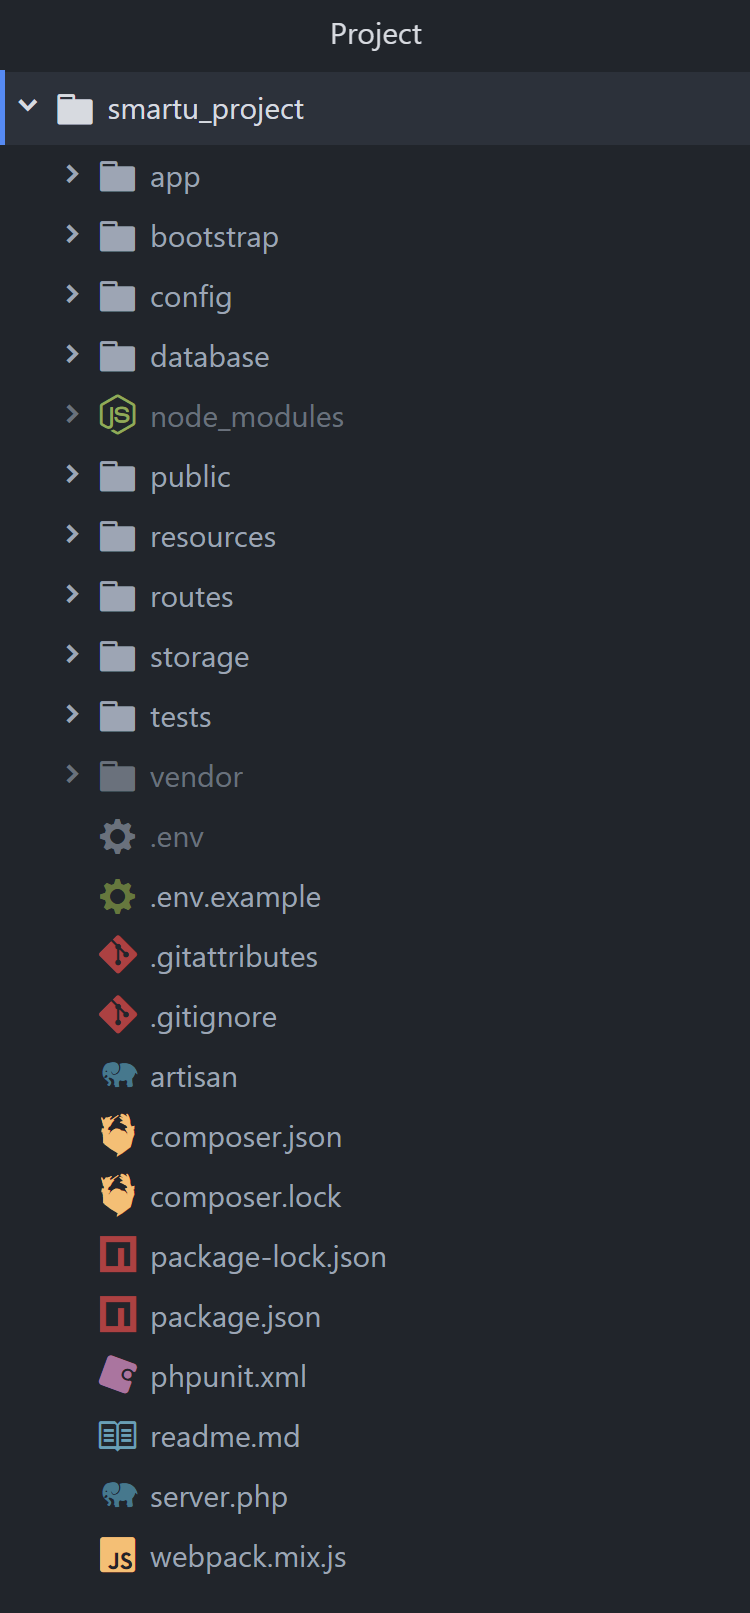
\includegraphics[scale=1.25]{directorios}
    \caption{Estructura de carpetas y ficheros del proyecto}
    \label{directorios}
\end{figure}

\subsection{Middlewares}
Laravel hace un extenso uso de los \textit{Middlewares}. Podemos definirlos como software intermediario que proporciona una capa de abstracción entre una aplicación y otra. En el caso de Laravel, nos proporciona por defecto una serie de middlewares que realizan varias tareas sin que nosotros tengamos que intervenir en ellas, liberando al programador de carga de trabajo.\\

Uno de los principales middleware que proporciona este framework es el de autenticación. Permite, por ejemplo, que un usuario autentificado en el sistema pueda realizar ciertas tareas y evita que aquellos que no lo están las puedan hacer, en cuyo caso los redigire a otra dirección que si tengan permitida. Otro middleware importante es el de la verificación del token CSRF, pero esto lo hablaremos con más detalle en el apartado de seguridad.

\subsubsection{Middleware de localización}
Con el objetivo de lograr que la aplicación web tuviera soporte \textbf{multilenguaje}, se ha hecho uso de un middleware personalizado que captura los parámetros de la URL y detecta si existe un código de idioma correcto, y en caso de no tenerlo, le añade el del idioma por defecto de la aplicación. Como se puede comprobar, los middlewares nos permiten delegar ciertas tareas para no tener que preocuparnos de nada y poder continuar el desarrollo.

\subsection{Patrones de diseño}
El uso de patrones de diseño es muy recomendable a la hora de desarrollar software. Laravel, por su funcionamiento interno, logra aplicar el patrón MVC mencionado anteriormente, pero no es el único que encontramos. Existen más patrones de diseño que se aplican para determinadas características, como por ejemplo:

\begin{description}
    \item [Builder] El patrón Builder permite separar la creación de un objeto complejo de su representación, con el fin de que el mismo proceso de construcción pueda usarse para crear diferentes representaciones. En Laravel podemos tomar como ejemplo la clase \textit{AuthManager}, que hereda de \textit{Manager}, siendo esta última la clase Builder que se encarga de construir los componentes seguros necesarios para almacenar informaciónde autentificación, ya sea en una variable de sesión o en una cookie.
    \item [Factoría] Este patrón permite definir una interfaz común de creación de objetos, pero deja a las subclases que sean ellas las que decidan qué objeto es el que quieren instanciar. Laravel hace un extenso uso de este patrón, por ejemplo, a la hora de crear conjuntos de reglas de validación de datos (usados habitualmente para comprobar los que se reciben a través de un formulario).
    \item [Estrategia] El patrón Estrategia o también conocido como \textit{Policy}, define una familia de algoritmos y los encapsula cada uno, haciendo que estos puedan ser reutilizados en cualquier momento.
    \item [Fachada] El patrón Fachada proporciona una interfaz unificada a un conjunto de interfaces de un subsistema. La fachada define una interfaz de alto nivel que hace que el subsistema sea más sencillo de usar. Laravel está construido con el uso de este patrón en casi todas partes, agrupando funcionalidades complejas en unas más simples de usar.
\end{description}

\section{Pruebas}
Para realizar la fase de pruebas de este proyecto, se ha seguido el proceso habitual de una \textbf{metodología ágil}, es decir, probar que las funcionalidades de la aplicación web funcionan correctamente en todos los posibles casos de uso. En concreto, se ha seguido el siguiente proceso:

\begin{itemize}
    \item El desarrollo se ha realizado implementando en primer lugar las \textbf{funcionalidades \textit{core}} o ensenciales de la aplicación, es decir, la gestión de los usuarios y los proyectos, así como la gestión de los diferentes idiomas que pueda haber disponibles.\\
    Se ha garantizado mediante pruebas que en este punto es posible crear usuarios y proyectos, y los usuarios invitados (no registrados) sólo pueden hacer operaciones de consulta.\\
    También se ha garantizado que el cambio de idioma de la aplicación se hace correctamente.
    \item Tras la funcionalidad esencial, se han implementado las \textbf{pequeñas funcionalidades} que no presentan un fuerte acoplamiento con otras y que no dependen del funcionamiento de éstas, de modo que se puede garantizar más rápidamente su correcto funcionamiento.\\
    Entre las funcionalidades que se consideran ``auto-contenidas'' encontramos los comentarios de un proyecto, los avances, los ``Buena Idea'', las áreas y las especialidades.
    \item Por último, una vez que se ha realizado todo lo necesario para probar la funcionalidad esencial y las pequeñas funcionalidades auto-contenidas, se procedió a la implementación de las \textbf{funcionalidades más complejas} que requerían de la interacción entre otros componentes de la aplicación. Cada funcionalidad se iba probando en todos los posibles casos de uso. Aquí se incluye toda la funcionalidad relativa a las vacantes y las solicitudes para incorporarse como integrantes de un proyecto, y las notificaciones.
\end{itemize}

Debido a los problemas de tiempo que he tenido para realizar este proyecto, no he podido realizar pruebas más exahustivas de la implementación, o incluso pruebas unitarias. Para futuras ampliaciones de este proyecto (ya que se espera una continuación del mismo), sería apropiado realizar una colección de pruebas que se pudieran ejecutar de forma automatizada antes de proceder a incrementar el conjunto de funcionalidades de la aplicación web.

\section{Herramientas de desarrollo}
Para el desarrollo de este proyecto he utilizado el siguiente conjunto de herramientas y programas de desarrollo:

\begin{itemize}
    \item Laravel 5.5 con la versión 7 del lenguaje PHP.
    \item Servidor de pruebas XAMPP con instalación de Apache y MariaDB.
    \item Editor de texto Atom 1.19.
    \item Draw.io (diagramas del proyecto).
    \item Windows 10 Pro Versión 1703.
\end{itemize}

\subsection{Capturas de pantalla de la aplicación}
En esta sección se muestran una serie de capturas de pantalla de la aplicación que muestran lo que se ha implementado hasta ahora. Como se ha mencionado anteriormente, y se remarca en el capítulo \ref{ch:conclusiones}, aun quedan funcionalidades por implementar, que en sucesivas iteraciones del proyecto deberán ser terminadas.\\

Para poder ilustrar la aplicación y ver cómo quedan algunas de sus secciones, se ha rellenado con datos de ejemplo y el uso del \textit{Lorem Ipsum} como relleno para los cuadros de texto.\\

En las imágenes \ref{welcome} y \ref{dashboard} podemos ver la pantalla de bienvenida de SmartU y la página principal de proyectos/comentarios destacados, así como los últimos proyectos publicados y una zona para buscar por diferentes áreas.\\

\begin{figure}
    \centering
    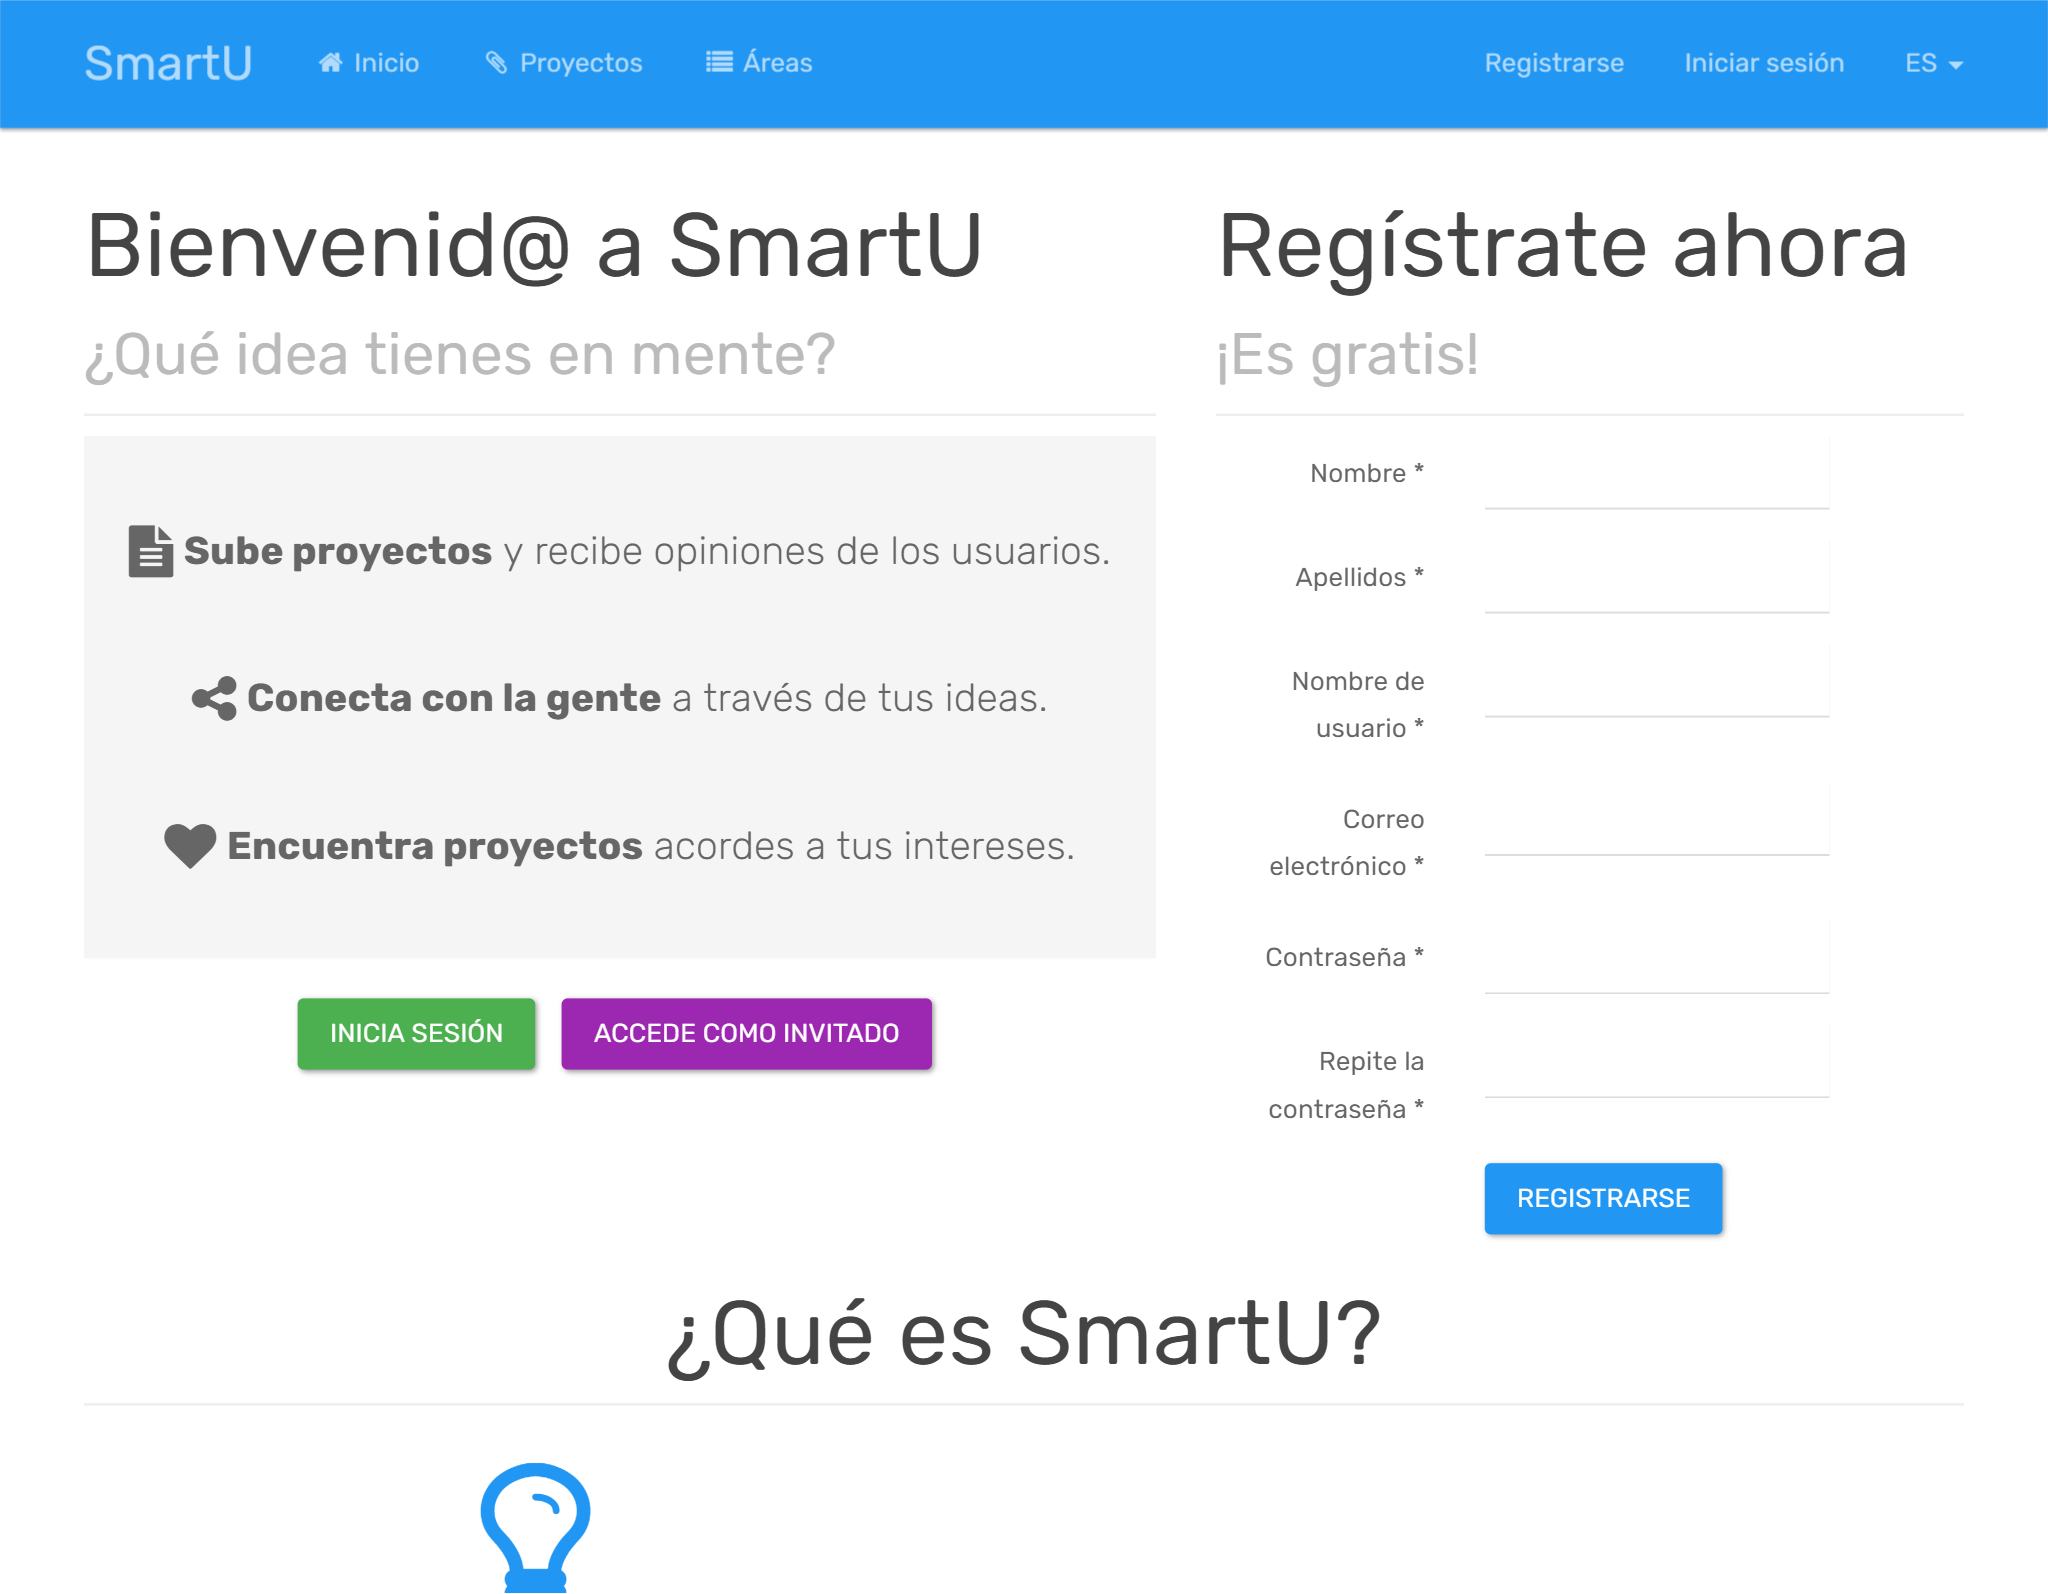
\includegraphics[scale=0.16]{welcome}
    \caption{Página de bienvenida de SmartU}
    \label{welcome}
\end{figure}

\begin{figure}
    \centering
    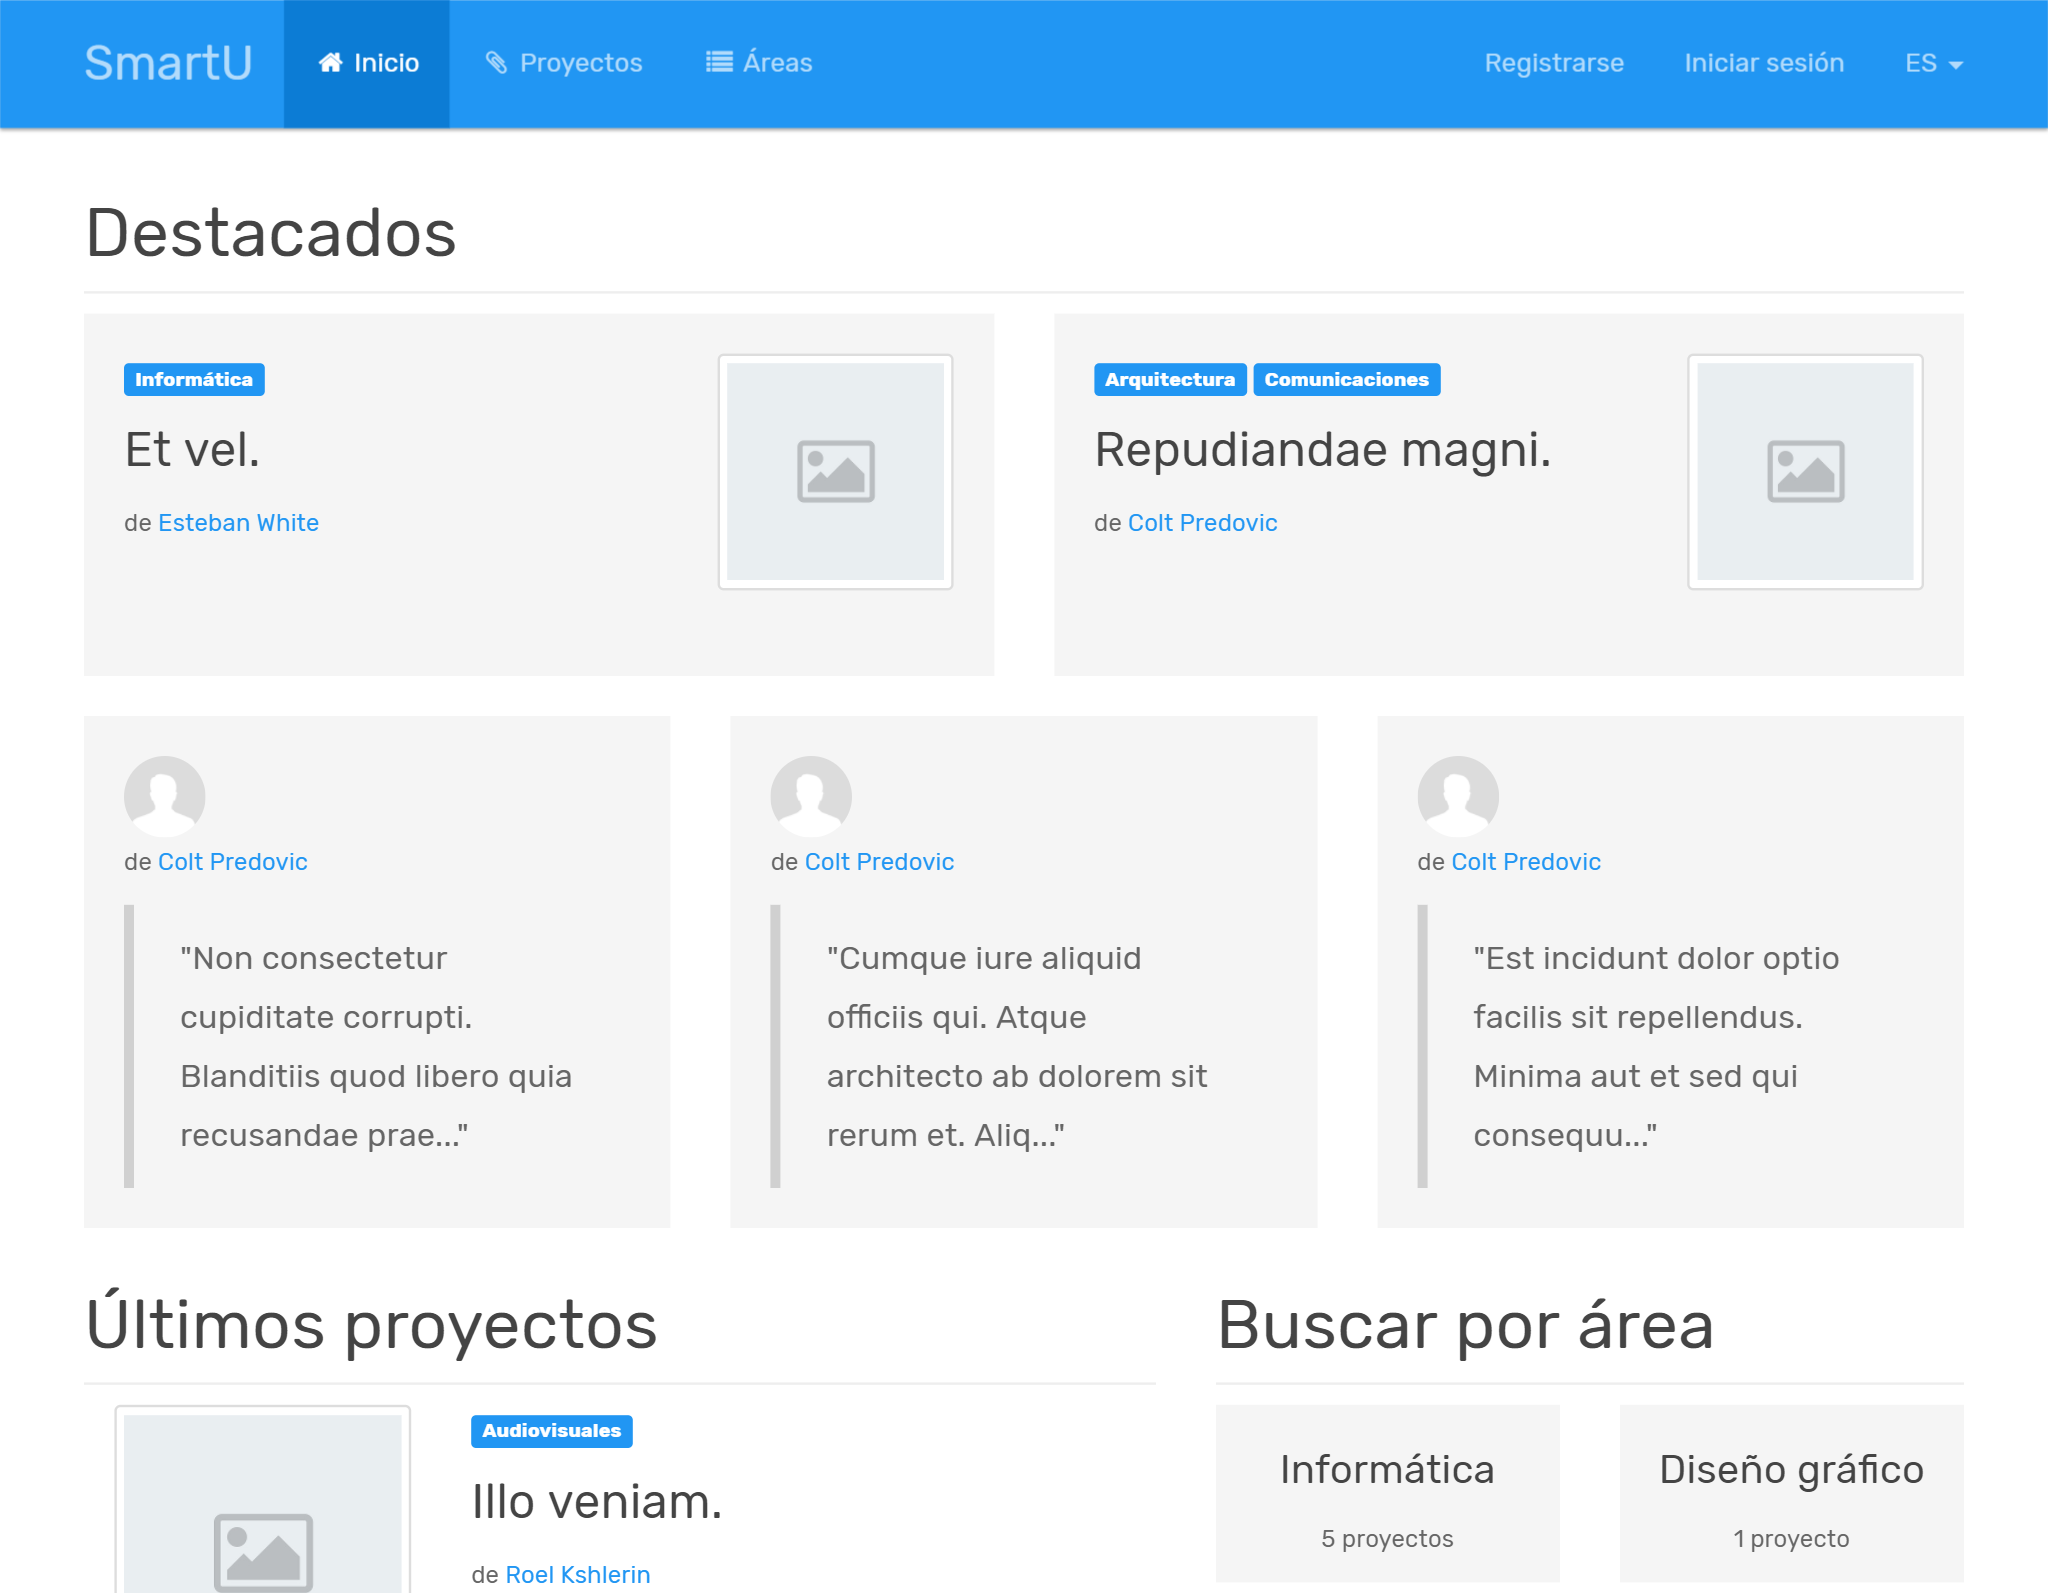
\includegraphics[scale=0.16]{dashboard}
    \caption{Página inicial de SmartU (Destacados)}
    \label{dashboard}
\end{figure}

En la figura \ref{dashboardenglish} se puede apreciar la característica de multilenguaje de la aplicación en la misma página de destacados. Cualquier usuario puede entrar y ver los proyectos, pero para poder interactuar más en SmartU, como por ejemplo dejar un comentario, o publicar un proyecto, nuevo, primero hay que registrarse, tal y como se ve en la imagen \ref{register}.\\

\begin{figure}
    \centering
    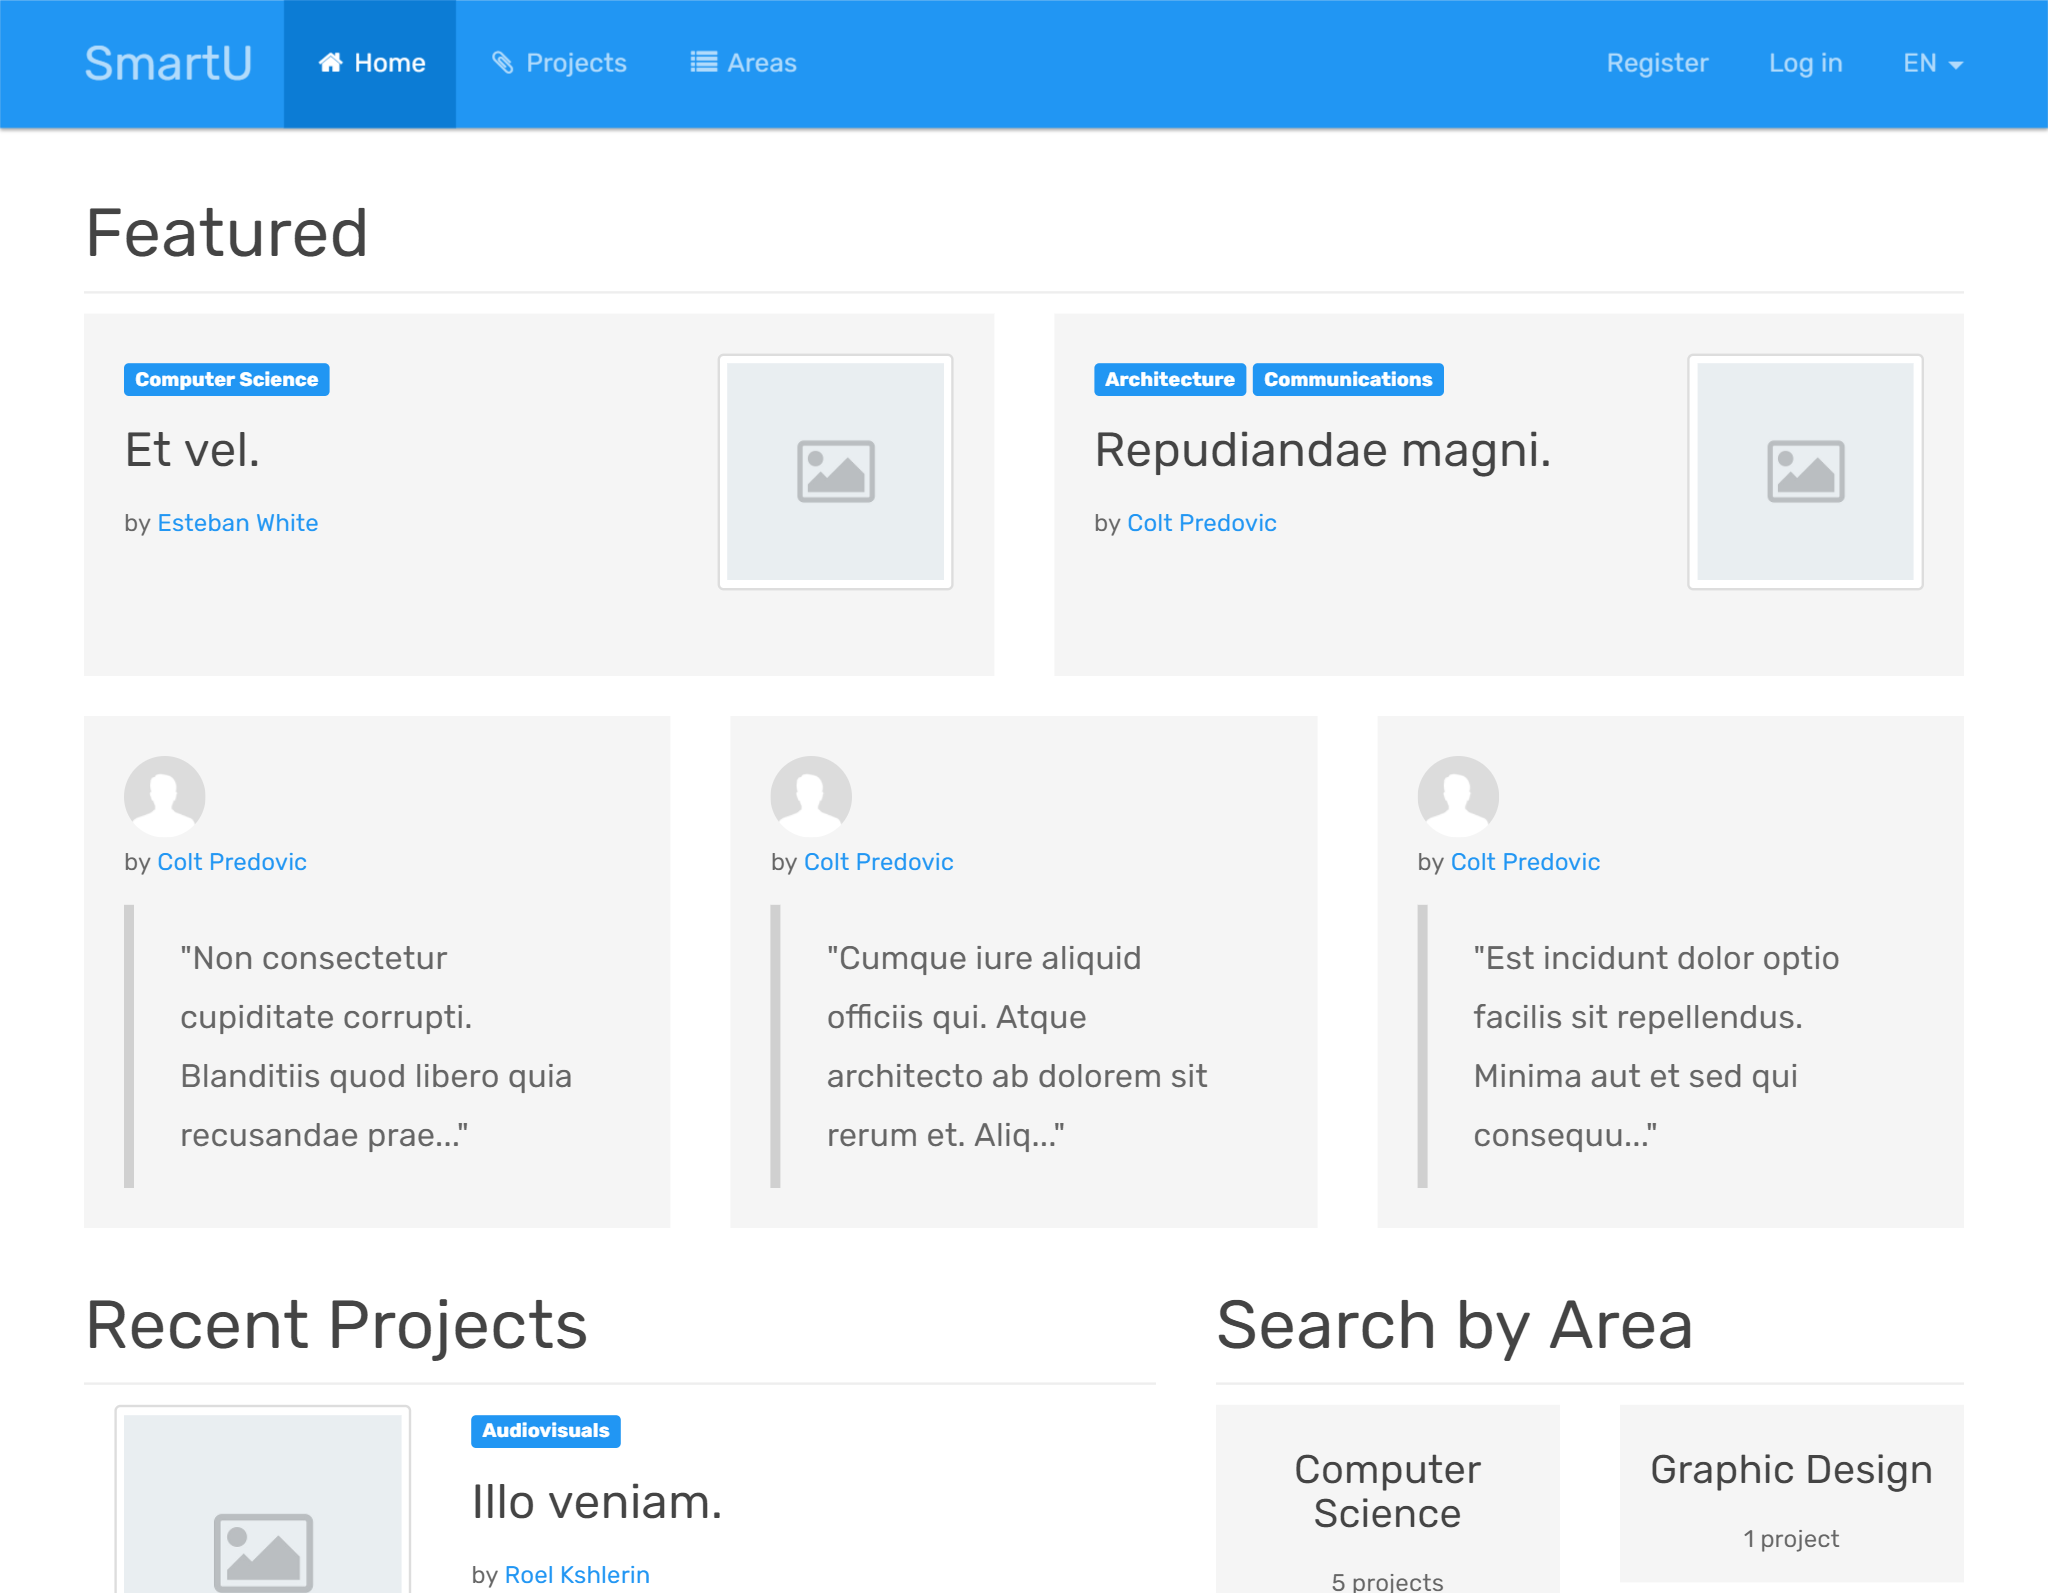
\includegraphics[scale=0.16]{dashboardenglish}
    \caption{Página inicial de SmartU con el idioma en inglés}
    \label{dashboardenglish}
\end{figure}

\begin{figure}
    \centering
    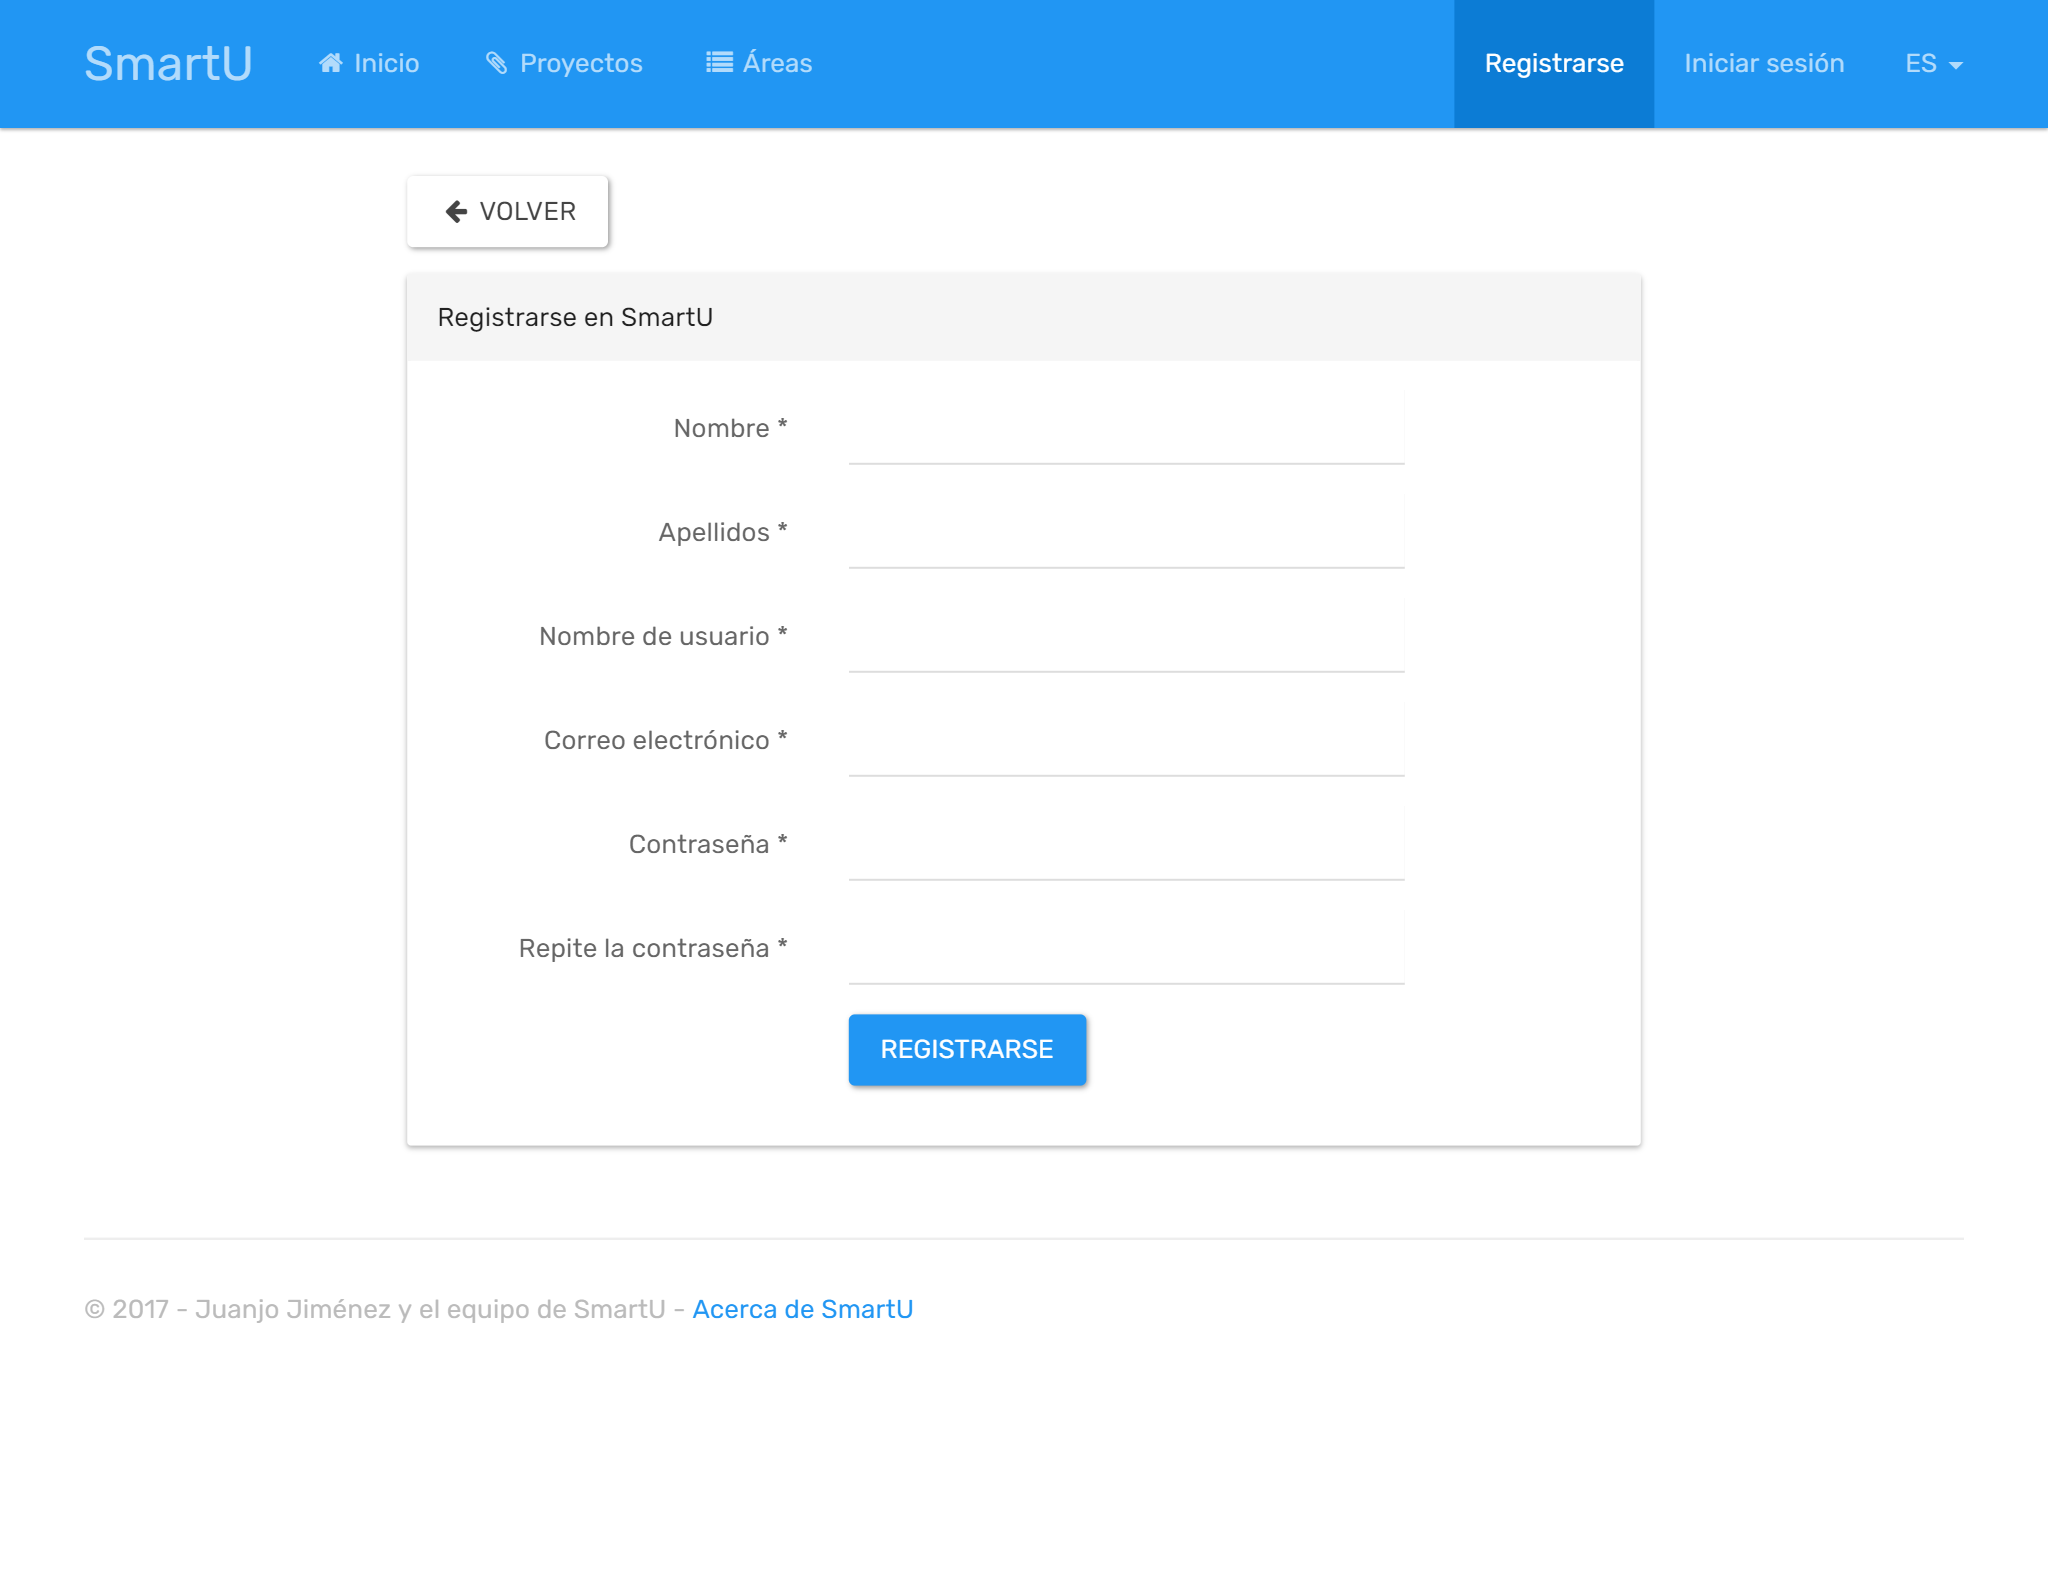
\includegraphics[scale=0.16]{register}
    \caption{Página de registro de un nuevo usuario}
    \label{register}
\end{figure}

En las imágenes \ref{projects}, \ref{project} y \ref{progress} se ve las secciones de \textit{Todos los proyectos}, \textit{Detalle de un proyecto} y la sección de avances (hitos, progresos que se hacen en el proyecto), así como los comentarios que otros usuarios han dejado en el proyecto.

\begin{figure}
    \centering
    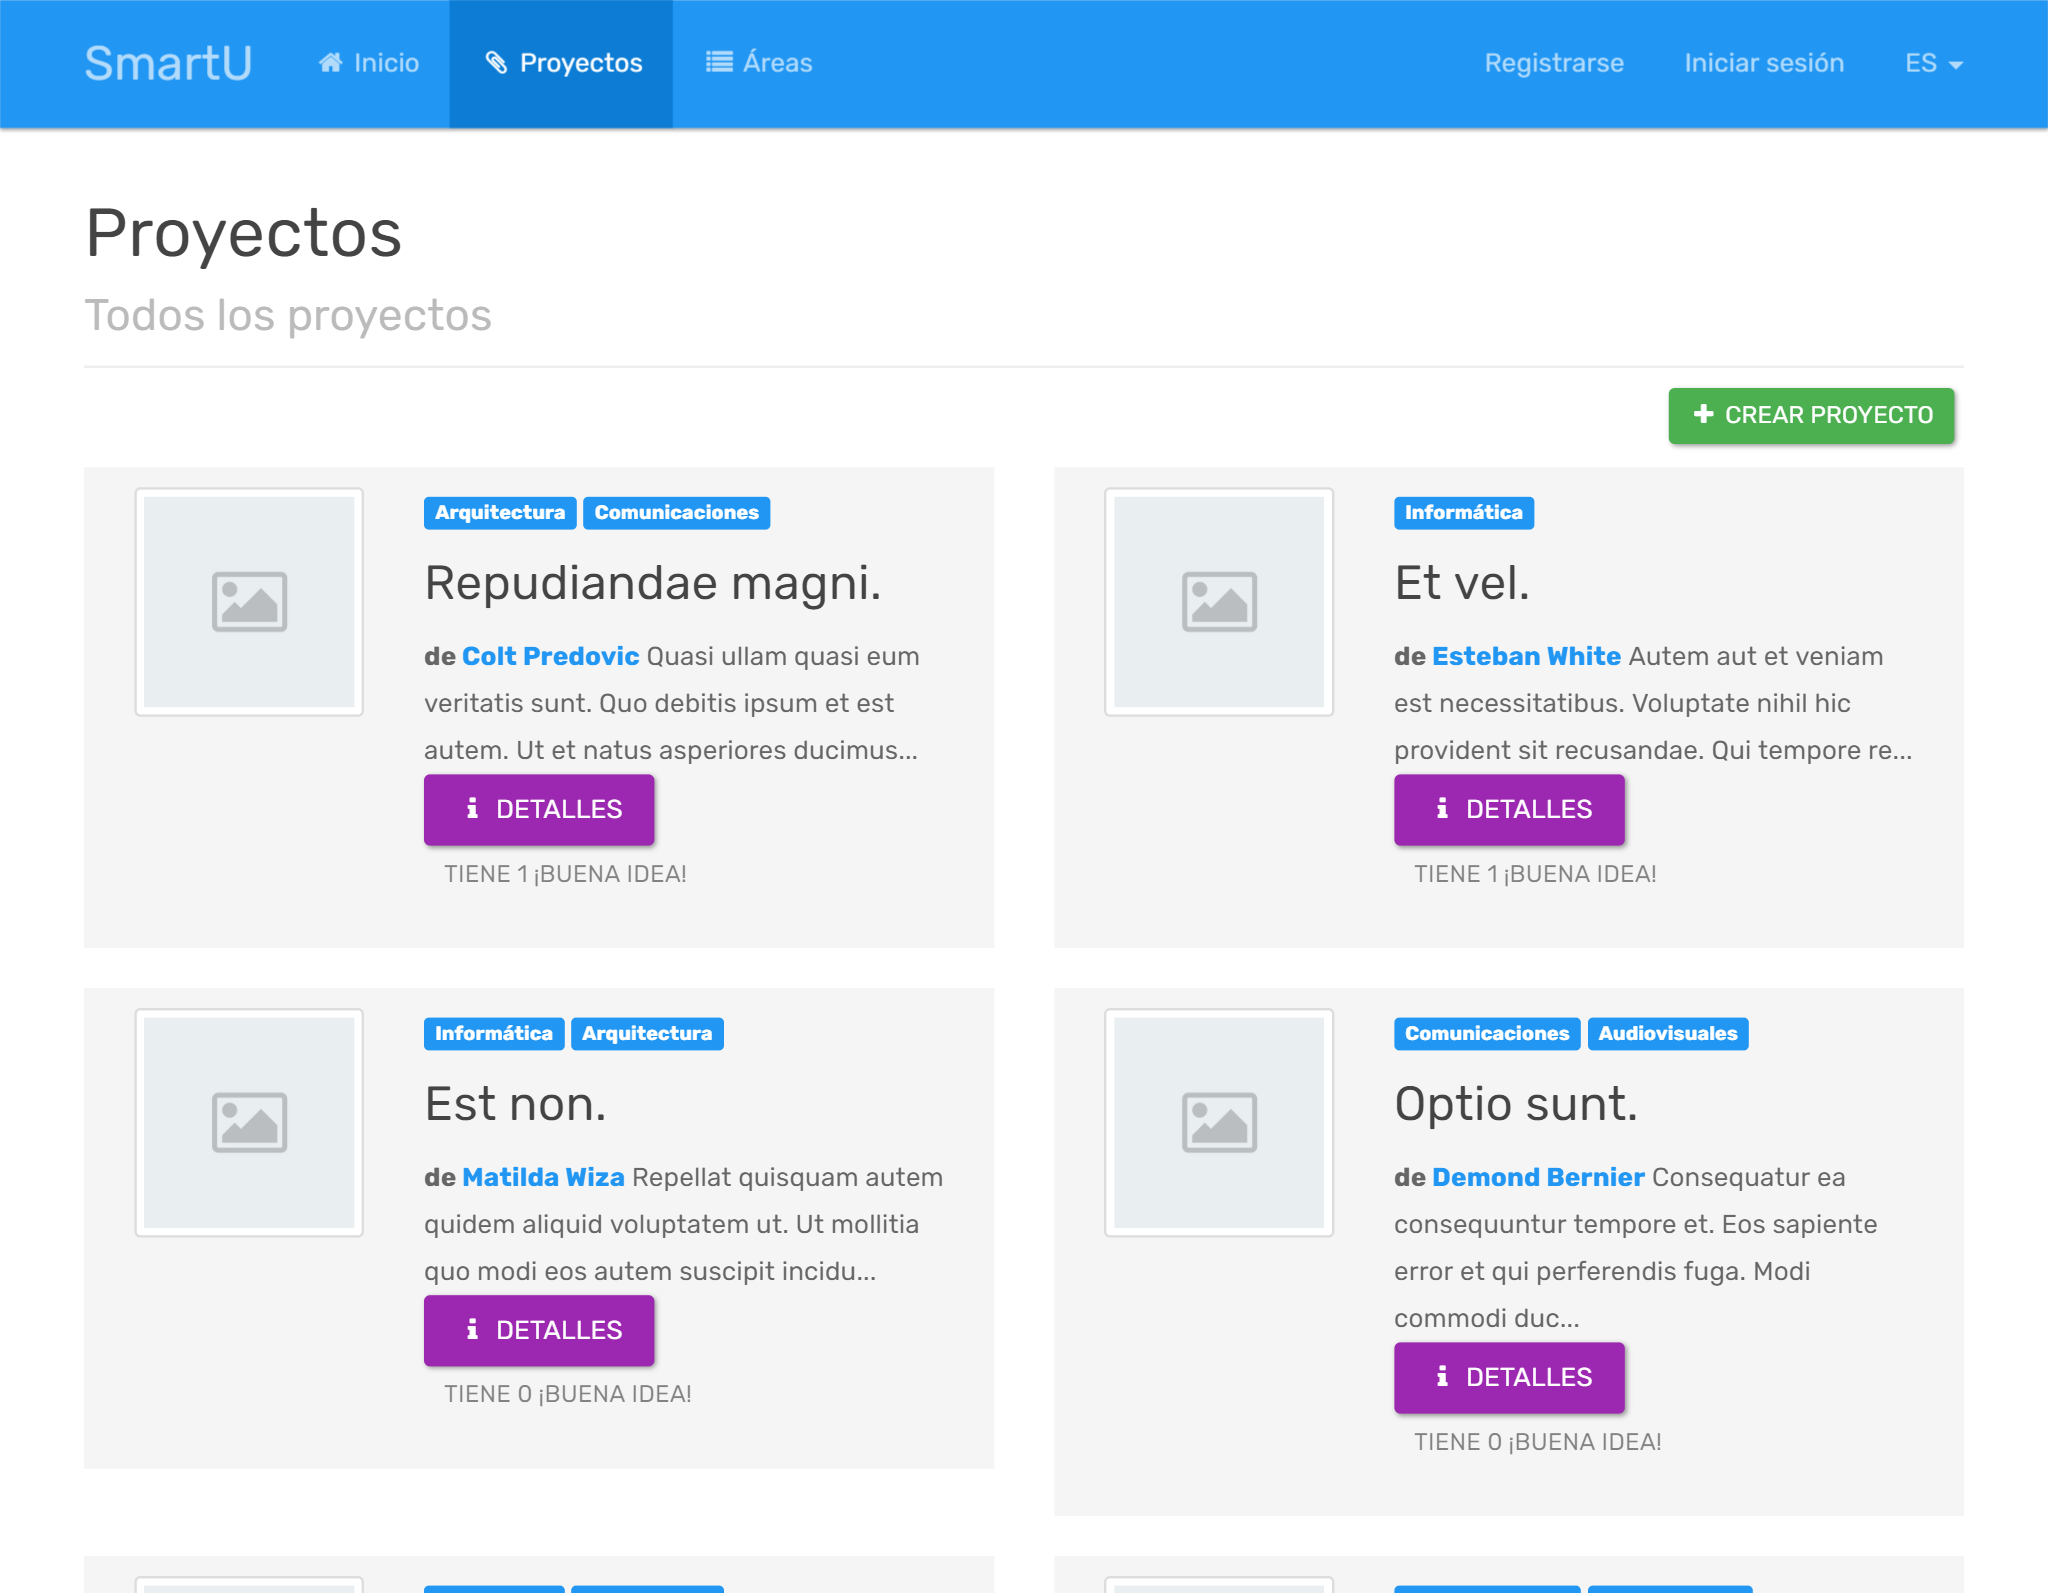
\includegraphics[scale=0.16]{projects}
    \caption{Listado de todos los proyectos}
    \label{projects}
\end{figure}

\begin{figure}
    \centering
    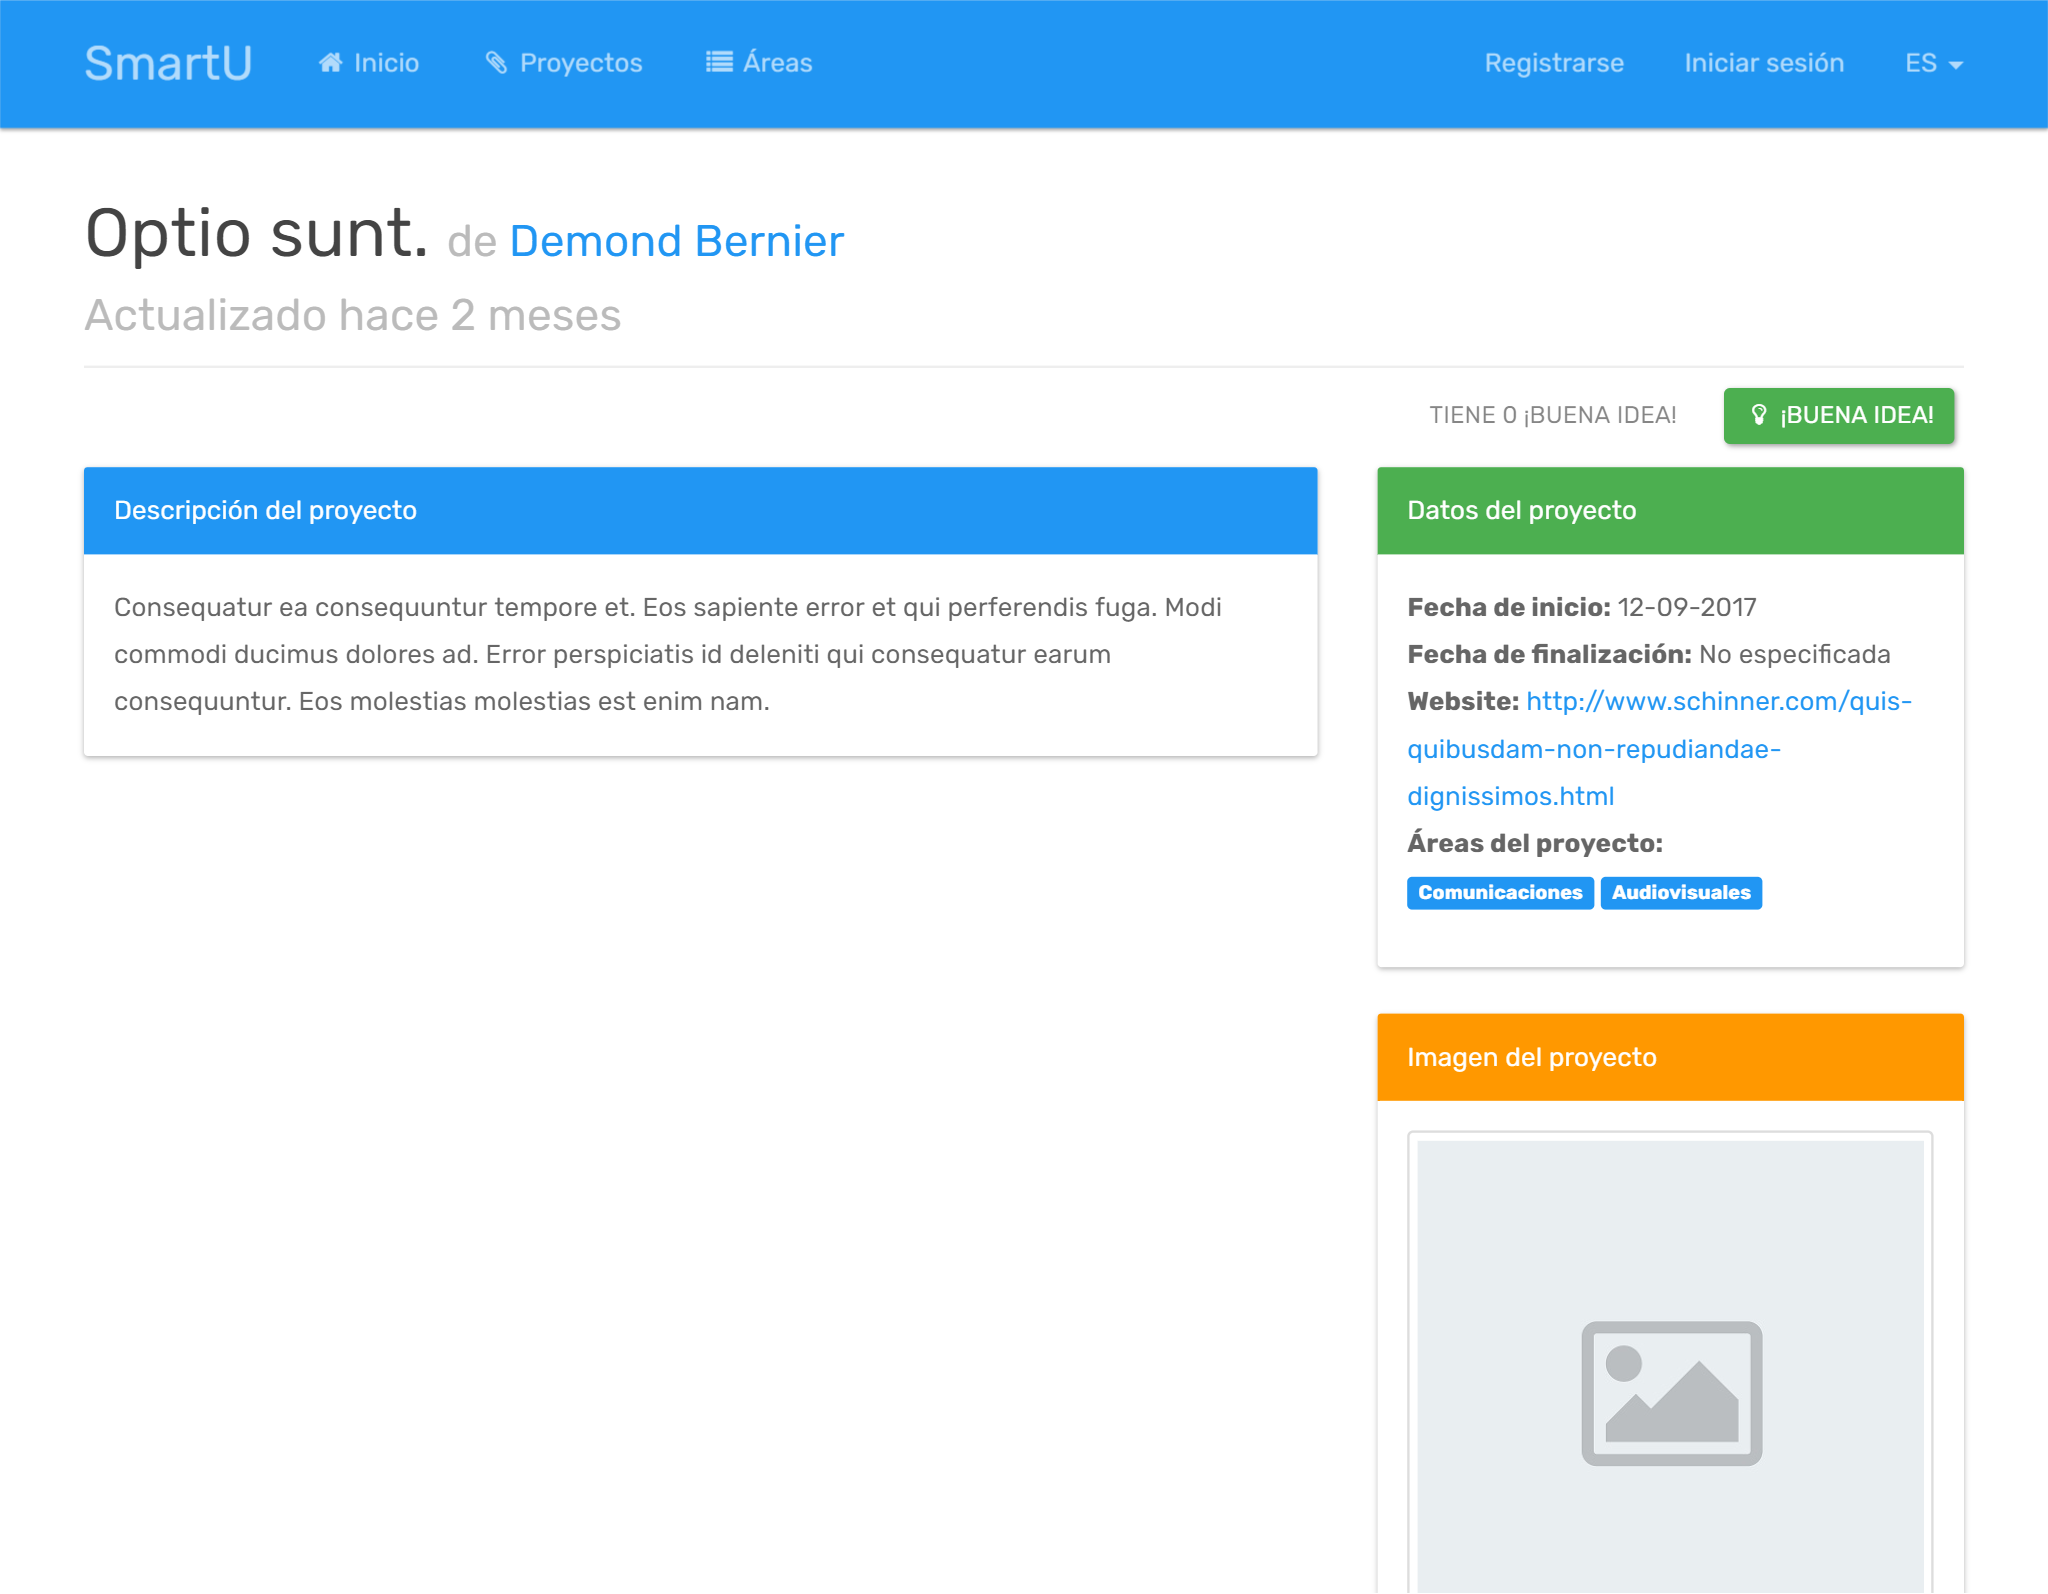
\includegraphics[scale=0.16]{project}
    \caption{Vista de detalles de un proyecto}
    \label{project}
\end{figure}

\begin{figure}
    \centering
    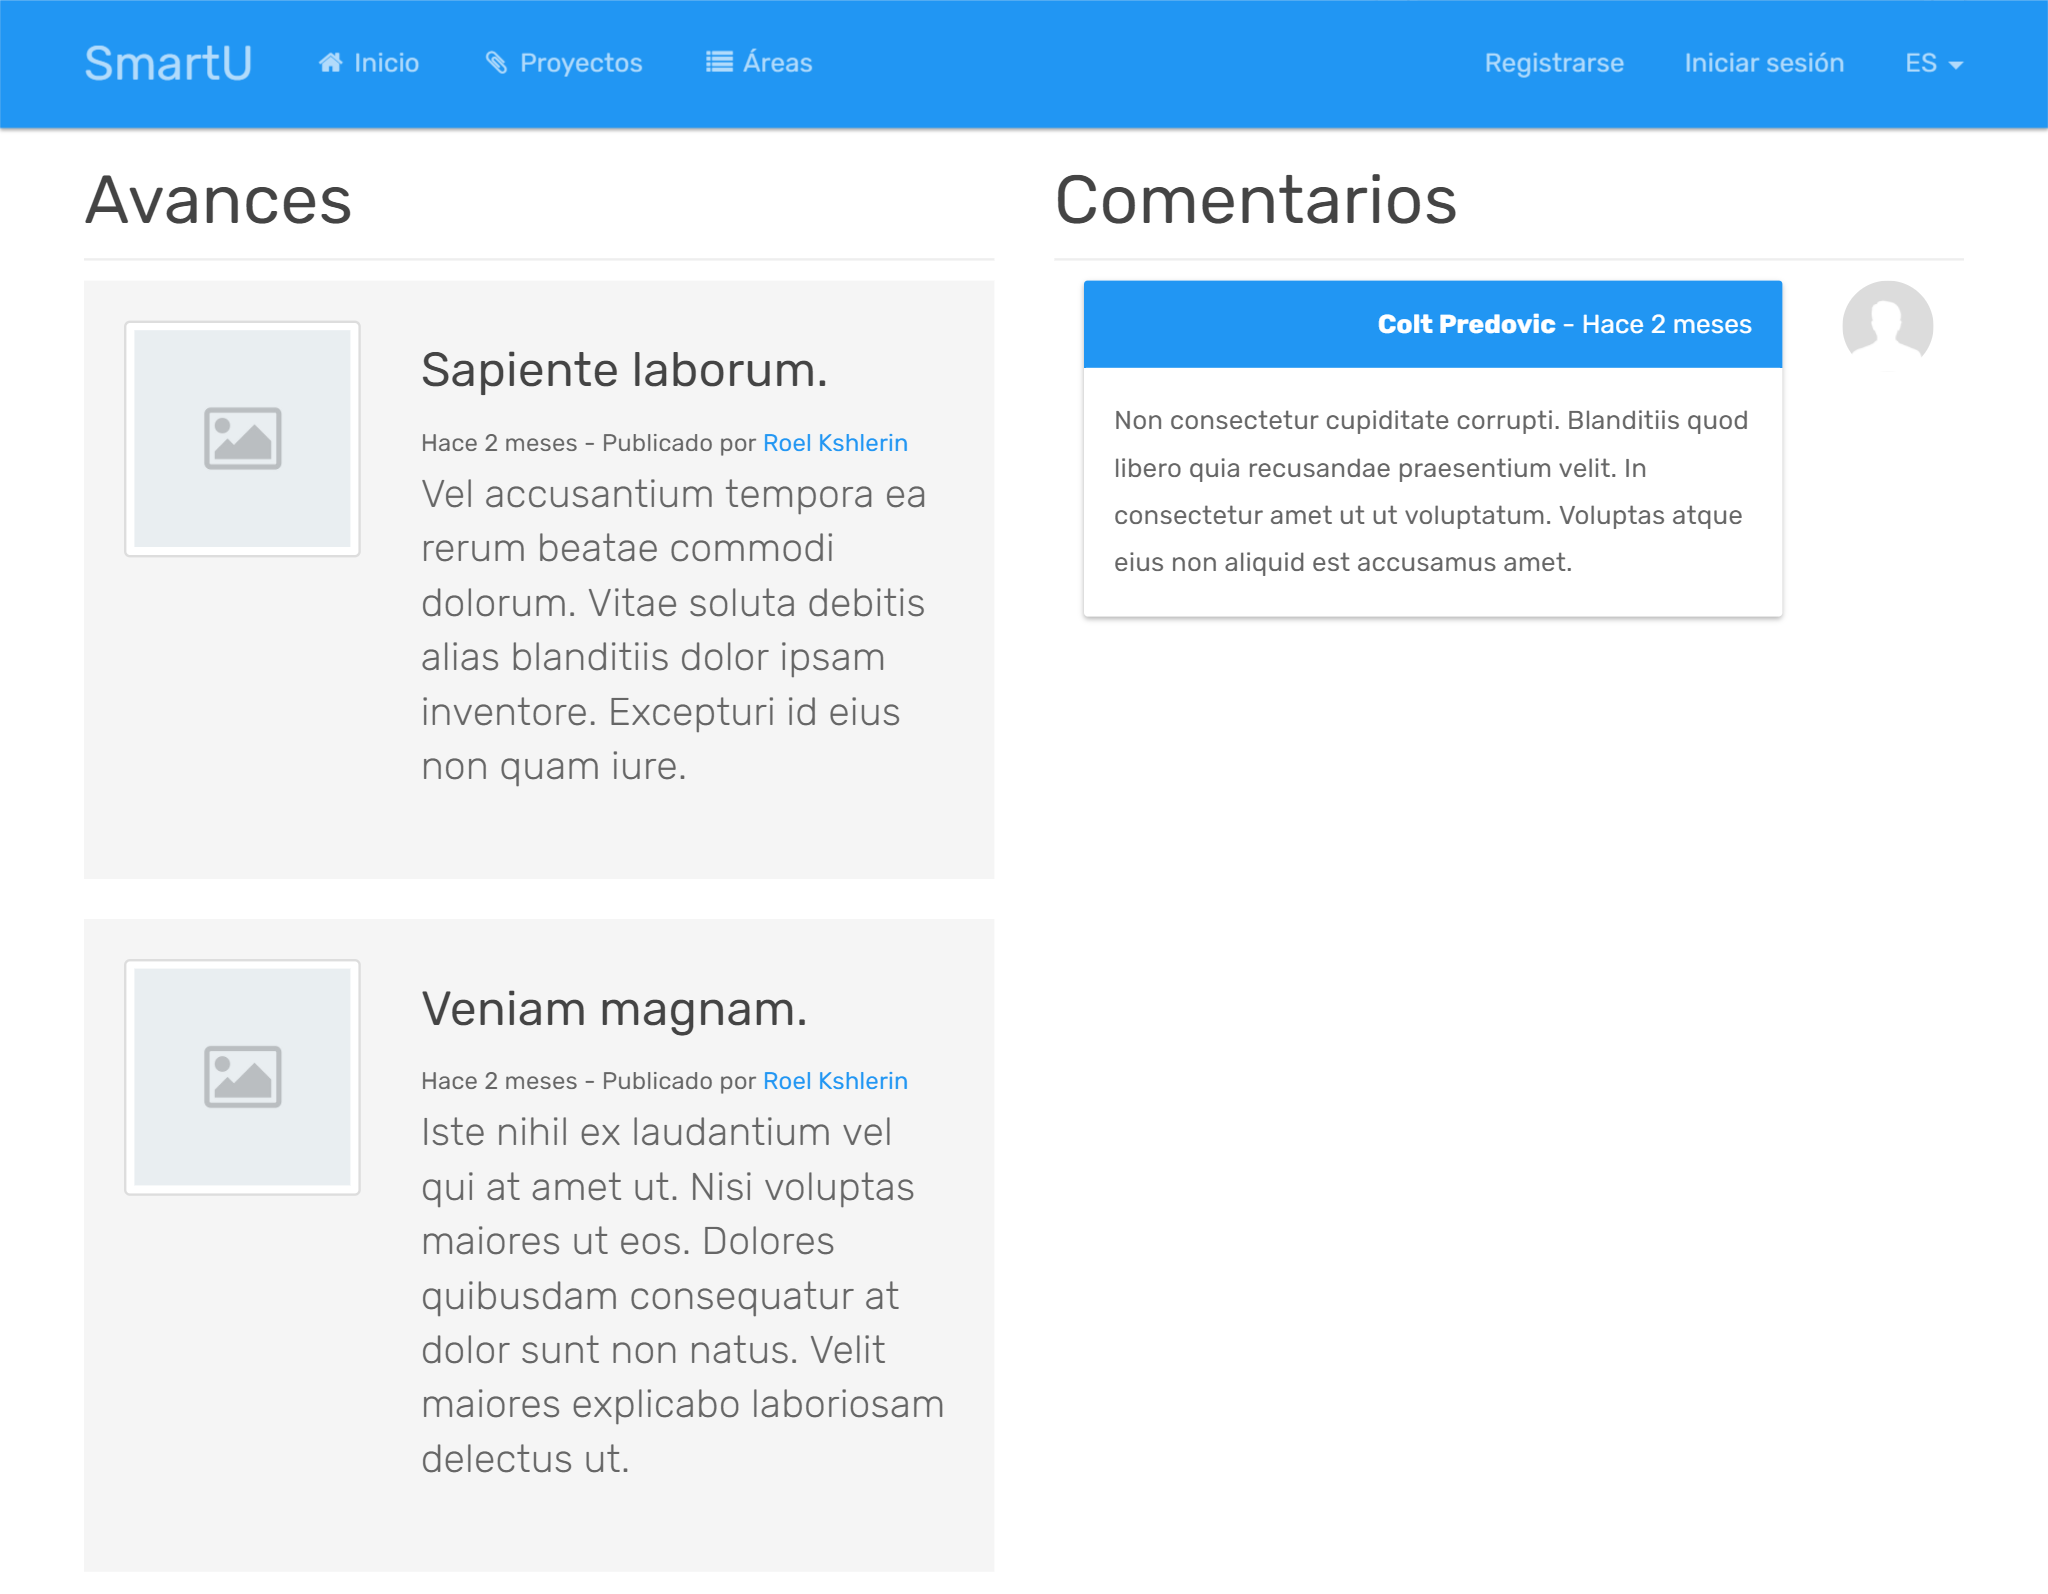
\includegraphics[scale=0.16]{progress}
    \caption{Vista de avances y comentarios de un proyecto}
    \label{progress}
\end{figure}
